% ***************************************************************************************************
%
%	Szablon pracy magisterskiej dla Politechniki Wrocławskiej w wersji dwustronnej.
%	Autor:	Tomasz Strzałka
% Koretkta i dostosowanie do wymogów WIT 3.12.2021: dr inż. Anna Lauks-Dutka
%
% ***************************************************************************************************

% Styl dwustronny z domyślną wielkością czcionki 10pt oraz oddzieloną stroną tytułową (titlepage).
% Domyślnie rodziały rozpoczynają się na stronie prawej (openright).
\documentclass[10pt]{book}
\usepackage{times}


% ***************************************************************************************************
% Ustawienia języka
% ***************************************************************************************************

% Podstawowe ustawienia języka, według którego formatowany będzie dokument
\usepackage[polish]{babel}

% Pakiet babel dla polskiego języka powoduje konflikt z pakietem amssymb.
% Polecenie '\lll' definiują oba pakiety - porządana jest druga definicja.
\let\lll\undefined

% W przypadku wielojęzykowości ustawia główny język dokumentu
\selectlanguage{polish}

% Kodowanie dokumentu
\usepackage[utf8]{inputenc}

% Dowolny rozmiar czcionek, kodowanie znaków
\usepackage{lmodern}

% Polskie wcięcia akapitów
\usepackage{indentfirst}

% Polskie łamanie wyrazów
\usepackage[plmath]{polski}

% Przecinek w wyrażeniach matematycznych zamiast kropki
\usepackage{icomma}

% Polskie formatowanie typograficzne
\frenchspacing

% Zapewnia liczne usprawnienia wyświetlania i organizacji matematycznych formuł. 
\usepackage{amsmath}

% Wprowadza rozszerzony zestaw symboli m.in. \leadsto
\usepackage{amssymb}

% Dodatkowa, ,,kręcona'' czcionka matematyczna
\usepackage{mathrsfs}

% Dodatkowe wsparcie dla środowiska mathbb, które nie wspiera domyślnie cyfr (\mathbb{})
\usepackage{bbold}

% Fixes/improves amsmath
\usepackage{mathtools}

% PROLOG kod źródłowy
\usepackage{minted}


% ***************************************************************************************************
% Kolory  
% ***************************************************************************************************

% Umożliwia kolorowanie poszczególnych komórek tabeli
\usepackage[table]{xcolor}% http://ctan.org/pkg/

% Umożliwia łatwą zmianę koloru linii w tabeli
\usepackage{tabu}

% Umożliwia rozszerzoną kontrolę nad kolorami.
\usepackage{xcolor}

% Definicje kolorów
\definecolor{lgray}{HTML}{9F9F9F}
\definecolor{dgray}{HTML}{5F5F5F}
% lgray				-	nazwa nowo zdefiniowanego koloru
% HTML				-	model kolorów
% CCCCCC			-	wartość koloru zgodna z modelem

% ***************************************************************************************************
% Algorytmy 
% ***************************************************************************************************

% Udostępnia środowisko do konstruowania pseudokodów
\usepackage[ruled,vlined,linesnumbered,longend,algochapter]{algorithm2e}
% ruled	- poziome kreski na początku i końcu algorytmu, podpis na górze oddzielony również kreską poziomą
% vlined - pionowe kreski łączące początek polecenia z jego końcem
% linesnumbered	- numerowanie kolejnych wierszy algorytmu
% longend - długie końcówki np. ifend, forend itd.
% algochapter - numeracja z rozdziałami

% Zamiana nazwy środowiska z domyślnej "Algorithm X" na "Pseudokod X"
\newenvironment{pseudokod}[1][htb]{
	\renewcommand{\algorithmcfname}{Pseudokod}
	\begin{algorithm}[#1]%
	}{
\end{algorithm}
}

% Zmiana rozmiaru komentarzy
\newcommand\algcomment[1]{
	\footnotesize{#1}
}

% Ustawienie zadanego stylu dla komentarzy
\SetCommentSty{algcomment}

% Wyśrodkowana tylda
\usepackage{textcomp}%
\newcommand{\textapprox}{\raisebox{0.5ex}{\texttildelow}}

% Listowanie kodów źródłowych
\usepackage{listings} 
\renewcommand{\lstlistingname}{Kod źródłowy} % Polska nazwa listingu
\renewcommand\listingscaption{Kod źródłowy}


% Definicje pecjalnych znaków, które nie są obsługiwane w środowisku listing
\lstset{literate=
	{ż}{{\.{z}}}1	{ź}{{\'{z}}}1
	{ć}{{\'{c}}}1	{ń}{{\'{n}}}1
	{ą}{{\c a}}1	{ś}{{\'{s}}}1
	{ł}{{\l}}1		{ę}{{\c{e}}}1
	{ó}{{\'{o}}}1	{á}{{\'a}}1
	{é}{{\'e}}1		{í}{{\'i}}1
	{ó}{{\'o}}1		{ú}{{\'u}}1
	{ù}{{\`u}}1		{Á}{{\'A}}1
	{É}{{\'E}}1		{Í}{{\'I}}1
	{Ó}{{\'O}}1		{Ú}{{\'U}}1
	{à}{{\`a}}1		{è}{{\'e}}1
	{ì}{{\`i}}1		{ò}{{\`o}}1
	{ò}{{\`o}}1		{À}{{\`A}}1
	{È}{{\'E}}1		{Ì}{{\`I}}1
	{Ò}{{\`O}}1		{Ò}{{\`O}}1
	{ä}{{\"a}}1		{ë}{{\"e}}1
	{ï}{{\"i}}1		{ö}{{\"o}}1
	{ü}{{\"u}}1		{Ä}{{\"A}}1
	{Ë}{{\"E}}1		{Ï}{{\"I}}1
	{Ö}{{\"O}}1		{Ü}{{\"U}}1
	{â}{{\^a}}1		{ê}{{\^e}}1
	{î}{{\^i}}1		{ô}{{\^o}}1
	{û}{{\^u}}1		{Â}{{\^A}}1
	{Ê}{{\^E}}1		{Î}{{\^I}}1
	{Ô}{{\^O}}1		{Û}{{\^U}}1
	{œ}{{\oe}}1		{Œ}{{\OE}}1
	{æ}{{\ae}}1		{Æ}{{\AE}}1
	{ß}{{\ss}}1		{ç}{{\c c}}1
	{Ç}{{\c C}}1	{ø}{{\o}}1
	{å}{{\r a}}1	{Å}{{\r A}}1
	{€}{{\EUR}}1	{£}{{\pounds}}1
}

% ***************************************************************************************************
% Marginesy 
% ***************************************************************************************************

% Ustawienia rozmiarów stron i ich marginesów
%korekta ALD - dodatkowe 0.5cm na oprawę z lewej
%\usepackage[headheight=18pt, top=25mm, bottom=25mm, left=25mm, right=25mm]{geometry}
\usepackage[headheight=18pt, top=25mm, bottom=25mm, left=30mm, right=25mm]{geometry}
% headheight		-	wysokość tytułów
% top				-	margines górny
% bottom			-	margines dolny
% left				-	margines lewy
% right				-	margines prawy

% Usunięcie górnego marginesu dla środowisk
\makeatletter
\setlength\@fptop{0\p@}	
\makeatother

% ***************************************************************************************************
% Styl 
% ***************************************************************************************************

% Definiuje środowisko 'titlingpage', które zapewnia pełną kontrolę nad układem strony tytułowej.
\usepackage{titling}


% Umożliwia modyfikowanie stylu spisu treści
\usepackage{tocloft}	

\tocloftpagestyle{tableOfContentStyle}

% Definiowanie własnych stylów nagłówków i/lub stopek
\usepackage{fancyhdr}

% Domyślny styl dla pracy 
\fancypagestyle{custom}{
	\fancyhf{}									% wyczyść stopki i nagłówki
	\fancyhead[RO]{								% Prawy, nieparzysty nagłówek
%korekta ALD: 
%\hrulefill \hspace{16pt} \large Rozdział \thechapter
		\hrulefill \hspace{16pt} \large \ifnum \thechapter>0 {Rozdział \thechapter} \else{Wstęp}\fi
		\put(-472.1, 12.1){%
			\makebox(0,0)[l]{%
                
\includegraphics[width=0.05\textwidth]{pwr-logo}
			}
		}
		\put(-443,5.5){%
			\makebox(0,0)[l]{%
				\small Politechnika Wrocławska
			}
		}
	}
	\fancyhead[LE]{								% Lewy, parzysty nagłówek
%korekta ALD: 
%\large Rozdział \thechapter \hspace{16pt} \hrulefill 
        \large \ifnum \thechapter>0 {Rozdział \thechapter} \else{Wstęp}\fi \hspace{16pt} \hrulefill 
		\put(-22, 12.1){%
			\makebox(0,0)[l]{%
                %korekta ALD
				%
\includegraphics[width=0.05\textwidth]{pwr-logo}
                
\includegraphics[width=0.05\textwidth]{wit-logo}			}
		}
		\put(-210,5.5){%
			\makebox(0,0)[l]{%
%				\small Wydział Podstawowych Problemów Techniki
%Korekta ALD
\small Wydział Informatyki i Telekomunikacji
			}
		}
	}
	\fancyfoot[LE,RO]{							% Stopki
		\thepage
	}
	\renewcommand{\headrulewidth}{0pt}			% Grubość linii w nagłówku
	\renewcommand{\footrulewidth}{0.2pt}		% Grubość linii w stopce
}


% Domyślny styl dla bibliografii
\fancypagestyle{bibliographyStyle}{
	\fancyhf{}									% wyczyść stopki i nagłówki
	\fancyhead[RO]{								% Prawy, nieparzysty nagłówek
		\hrulefill \hspace{16pt} \large Dodatek \thechapter
		\put(-472.1, 12.1){%
			\makebox(0,0)[l]{%
	
\includegraphics[width=0.05\textwidth]{pwr-logo}
			}
		}
		\put(-443,5.5){%
			\makebox(0,0)[l]{%
				\small Politechnika Wrocławska
			}
		}
	}
	\fancyhead[LE]{								% Lewy, parzysty nagłówek
		\large Bibliografia \hspace{16pt} \hrulefill 
		\put(-22, 12.1){%
			\makebox(0,0)[l]{%
			%korekta ALD	\includegraphics[width=0.05\textwidth]{wppt-logo}
			
\includegraphics[width=0.05\textwidth]{wit-logo}
			}
		}
		\put(-210,5.5){%
			\makebox(0,0)[l]{%
			%korekta ALD
				%\small Wydział Podstawowych Problemów Techniki
				\small Wydział Informatyki i Telekomunikacji
			}
		}
	}
	\fancyfoot[LE,RO]{							% Stopki
		\thepage
	}
	\renewcommand{\headrulewidth}{0pt}			% Grubość linii w nagłówku
	\renewcommand{\footrulewidth}{0.2pt}		% Grubość linii w stopce
}

% Domyślny styl dla spisu tabel i rysunków
\fancypagestyle{listOfTablesStyle}{
	\fancyhf{}									% wyczyść stopki i nagłówki
	\fancyhead[RO]{								% Prawy, nieparzysty nagłówek
		\hrulefill \hspace{16pt} \large Spis tabel
		\put(-472.1, 12.1){%
			\makebox(0,0)[l]{%
			
\includegraphics[width=0.05\textwidth]{pwr-logo}
			}
		}
		\put(-443,5.5){%
			\makebox(0,0)[l]{%
				\small Politechnika Wrocławska
			}
		}
	}
	\fancyhead[LE]{								% Lewy, parzysty nagłówek
		\large Spis tabel \hspace{16pt} \hrulefill 
		\put(-22, 12.1){%
			\makebox(0,0)[l]{%

\includegraphics[width=0.05\textwidth]{wit-logo}
			}
		}
		\put(-210,5.5){%
			\makebox(0,0)[l]{%
				\small Wydział Informatyki i Telekomunikacji
			}
		}
	}
	\fancyfoot[LE,RO]{							% Stopki
		\thepage
	}
	\renewcommand{\headrulewidth}{0pt}			% Grubość linii w nagłówku
	\renewcommand{\footrulewidth}{0.2pt}		% Grubość linii w stopce
}

\fancypagestyle{listOfPlotsStyle}{
	\fancyhf{}									% wyczyść stopki i nagłówki
	\fancyhead[RO]{								% Prawy, nieparzysty nagłówek
		\hrulefill \hspace{16pt} \large Spis rysunków
		\put(-472.1, 12.1){%
			\makebox(0,0)[l]{%
			
\includegraphics[width=0.05\textwidth]{pwr-logo}
			}
		}
		\put(-443,5.5){%
			\makebox(0,0)[l]{%
				\small Politechnika Wrocławska
			}
		}
	}
	\fancyhead[LE]{								% Lewy, parzysty nagłówek
		\large Spis rysunków \hspace{16pt} \hrulefill 
		\put(-22, 12.1){%
			\makebox(0,0)[l]{%

\includegraphics[width=0.05\textwidth]{wit-logo}
			}
		}
		\put(-210,5.5){%
			\makebox(0,0)[l]{%
				\small Wydział Informatyki i Telekomunikacji
			}
		}
	}
	\fancyfoot[LE,RO]{							% Stopki
		\thepage
	}
	\renewcommand{\headrulewidth}{0pt}			% Grubość linii w nagłówku
	\renewcommand{\footrulewidth}{0.2pt}		% Grubość linii w stopce
}

% Domyślny styl dla dodatków
\fancypagestyle{appendixStyle}{
	\fancyhf{}									% wyczyść stopki i nagłówki
	\fancyhead[RO]{								% Prawy, nieparzysty nagłówek
		\hrulefill \hspace{16pt} \large Załącznik \thechapter
		\put(-472.1, 12.1){%
			\makebox(0,0)[l]{%

\includegraphics[width=0.05\textwidth]{pwr-logo}
			}
		}
		\put(-443,5.5){%
			\makebox(0,0)[l]{%
				\small Politechnika Wrocławska
			}
		}
	}
	\fancyhead[LE]{								% Lewy, parzysty nagłówek
		\large Załącznik \thechapter \hspace{16pt} \hrulefill 
		\put(-22, 12.1){%
			\makebox(0,0)[l]{%
%korekta ALD:				\includegraphics[width=0.05\textwidth]{wppt-logo}

\includegraphics[width=0.05\textwidth]{wit-logo}
			}
		}
		\put(-210,5.5){%
			\makebox(0,0)[l]{%
			%korekta ALD
				%\small Wydział Podstawowych Problemów Techniki
				\small Wydział Informatyki i Telekomunikacji
			}
		}
	}
	\fancyfoot[LE,RO]{							% Stopki
		\thepage
	}
	\renewcommand{\headrulewidth}{0pt}			% Grubość linii w nagłówku
	\renewcommand{\footrulewidth}{0.2pt}		% Grubość linii w stopce
}

% Osobny styl dla stron zaczynających rozdział/spis treści itd. (domyślnie formatowane jako "plain")
\fancypagestyle{chapterBeginStyle}{
	\fancyhf{}%
	\fancyfoot[LE,RO]{
		\thepage
	}
	\renewcommand{\headrulewidth}{0pt}
	\renewcommand{\footrulewidth}{0.2pt}
}

% Styl dla pozostałych stron spisu treści
\fancypagestyle{tableOfContentStyle}{
	\fancyhf{}%
	\fancyfoot[LE,RO]{
		\thepage
	}
	\renewcommand{\headrulewidth}{0pt}
	\renewcommand{\footrulewidth}{0.2pt}
}
% Formatowanie tytułów rozdziałów i/lub sekcji
\usepackage{titlesec}

% Formatowanie tytułów rozdziałów
\titleformat{\chapter}[hang]					% kształt
{
	\vspace{-10ex}
	%\Huge
	\large
	\bfseries
}												% formatowanie tekstu modyfikowanego elementu
{}												% etykieta występująca przed tekstem modyfikowanego elementu, niewidoczna w spisie treści
{
	10pt
}												% odstęp formatowanego tytułu od lewego marginesu/etykiety
{
    \large
	\bfseries
}												% formatowanie elementów przed modyfikowanym tytułem
[
\vspace{2ex}
%\rule{\textwidth}{0.4pt}
%\vspace{-4ex}
]												% dodatkowe formatowanie stosowane poniżej modyfikowanego tytułu


% Formatowanie tytułów sekcji
\titleformat{\section}[hang]					% kształt
{
	\vspace{2ex}
%	\titlerule\vspace{1ex}
	\large\bfseries
}												% formatowanie tekstu modyfikowanego elementu
{
	\thesection									% etykieta występująca przed tekstem modyfikowanego elementu, niewidoczna w spisie treści
}
{
	0pt
}												% odstęp formatowanego tytułu od lewego marginesu/etykiety
{
	\large
	\bfseries
}												% formatowanie elementów przed modyfikowanym tytułem


%ALD- ustawienia wielkości fontów dla rozdziałów i sekcji
\usepackage{sectsty}
%\chapterfont{\fontsize{14}{17.6}\selectfont}
\sectionfont{\fontsize{13}{16.8}\selectfont}
\subsectionfont{\fontsize{12}{15.6}\selectfont}

% ***************************************************************************************************
% Linki
% ***************************************************************************************************

% Umożliwia wstawianie hiperłączy do dokumentu
\usepackage{hyperref}							% Aktywuje linki

\hypersetup{
	colorlinks	=	true,					% Koloruje tekst zamiast tworzyć ramki.
	linkcolor		=	blue,					% Kolory: referencji,
        citecolor		=	blue,					% cytowań,
	urlcolor		=	blue					% hiperlinków.
}

% Do stworzenia hiperłączy zostanie użyta ta sama (same) czcionka co dla reszty dokumentu
\urlstyle{same}




% ***************************************************************************************************
% Linki
% ***************************************************************************************************

% Umożliwia zdefiniowanie własnego stylu wyliczeniowego
\usepackage{enumitem}

% Nowa lista numerowana z trzema poziomami
\newlist{myitemize}{itemize}{3}

% Definicja wyglądu znacznika pierwszego poziomu
\setlist[myitemize,1]{
	label		=	\textbullet,
	leftmargin	=	4mm}

% Definicja wyglądu znacznika drugiego poziomu
\setlist[myitemize,2]{
	label		=	$\diamond$,
	leftmargin	=	8mm}

% Definicja wyglądu znacznika trzeciego poziomu
\setlist[myitemize,3]{
	label		=	$\diamond$,
	leftmargin	=	12mm
}

% ***************************************************************************************************
% Inne pakiety
% ***************************************************************************************************

% Dołączanie rysunków
\usepackage{graphicx}
\graphicspath{ {./pictures/} }

%Lepsze pozycjonowanie
\usepackage{float}

% Figury i przypisy
\usepackage{caption}
\usepackage{subcaption}

% Umożliwia tworzenie przypisów wewnątrz środowisk
\usepackage{footnote}

% Umożliwia tworzenie struktur katalogów
\usepackage{dirtree}

% Rozciąganie komórek tabeli na wiele wierszy
\usepackage{multirow}

% Precyzyjne obliczenia szerokości/wysokości dowolnego fragmentu wygenerowanego przez LaTeX
\usepackage{calc}

% ***************************************************************************************************
% Matematyczne skróty
% ***************************************************************************************************

% Skrócony symbol liczb rzeczywistych
\newcommand{\RR}{\mathbb{R}}

% Skrócony symbol liczb naturalnych
\newcommand{\NN}{\mathbb{N}}

% Skrócony symbol liczb wymiernych
\newcommand{\QQ}{\mathbb{Q}}

% Skrócony symbol liczb całkowitych
\newcommand{\ZZ}{\mathbb{Z}}

% Skrócony symbol logicznej implikacji
\newcommand{\IMP}{\rightarrow}

% Skrócony symbol  logicznej równoważności
\newcommand{\IFF}{\leftrightarrow}

% ***************************************************************************************************
% Środowiska
% ***************************************************************************************************

% Środowisko do twierdzeń
\newtheorem{theorem}{Twierdzenie}[chapter]

% Środowisko do lematów
\newtheorem{lemma}{Lemat}[chapter]

% Środowisko do przykładów
\newtheorem{example}{Przykład}[chapter]

% Środowisko do wniosków
\newtheorem{corollary}{Wniosek}[chapter]

% Środowisko do definicji
\newtheorem{definition}{Definicja}[chapter]

% Środowisko do dowodów
\newenvironment{proof}{
	\par\noindent \textbf{Dowód.}
}{
\begin{flushright}
	\vspace*{-6mm}\mbox{$\blacklozenge$}
\end{flushright}
}

%ALD - nowe środowisko do streszczenia i abstractu
\newenvironment{streszczenie}{
	\par\noindent {\large \textbf{Streszczenie}\\[14pt]\indent}
}{}
\newenvironment{abstract}{
	\par\noindent {\large \textbf{Abstract}\\[14pt]\indent}
}{}

% Środowisko do uwag
\newenvironment{remark}{
	\bigskip \par\noindent \small \textbf{Uwaga.}
}{
\begin{small}
	\vspace*{4mm}
\end{small}
}

% ***************************************************************************************************
% Słownik
% ***************************************************************************************************

% Prawidłowe dzielenie wyrazów
\hyphenation{wszy-stkich ko-lu-mnę każ-da od-leg-łość
	dzie-dzi-ny dzie-dzi-na rów-nych rów-ny
	pole-ga zmie-nna pa-ra-met-rów wzo-rem po-cho-dzi
	o-trzy-ma wte-dy wa-run-ko-wych lo-gicz-nie
	skreś-la-na skreś-la-ną cał-ko-wi-tych wzo-rów po-rzą-dek po-rząd-kiem
	przy-kład pod-zbio-rów po-mię-dzy re-pre-zen-to-wa-ne
	rów-no-waż-ne bi-blio-te-kach wy-pro-wa-dza ma-te-ria-łów
	prze-ka-za-nym skoń-czo-nym moż-esz na-tu-ral-na cią-gu tab-li-cy
	prze-ka-za-nej od-po-wied-nio}

% ***************************************************************************************************
% Dokument
% ***************************************************************************************************

\frontmatter

\begin{document}

    \pagestyle{empty}
	\begin{titlingpage}
		\vspace*{\fill}
		\begin{center}
			\begin{picture}(430,500)
				\put(60,590){\makebox(0,0)[l]{\huge \textbf{Politechnika Wrocławska}}}
				\put(40,565){\makebox(0,0)[l]{\Large \textbf{Wydział Informatyki i Telekomunikacji}}}
                \put(0,550){\line(1,0){430}}
                \put(0,510){\makebox(0,0)[l]{\large Kierunek: \textbf{Informatyka Algorytmiczna (INA)}}}
                %\textbf{3 literowy kod kierunku}}}
                \put(0,490){\makebox(0,0)[l]{\large Specjalność: \textbf{-}}}                
                %\textbf{3 literowy kod specjalności}}}                
				\put(0,370){\begin{minipage}{0.9\textwidth}
				\centering
				\Huge \textsc{Praca Dyplomowa\\ Inżynierska}
                \end{minipage}
				}
% Tytuł pracy
				\put(0,230){\begin{minipage}{0.9\textwidth}
				\centering
				\LARGE \textbf{Implementacja programu GRAPHPLAN do planowania akcji z wykorzystaniem programowania ograniczeń}
                \end{minipage}
				}
% Autor pracy
				\put(0,170){\begin{minipage}{0.9\textwidth}
				\centering
				\Large {
				Radosław Wojtczak
				}
				\end{minipage}
				}
% dane promotora
				\put(0,90){\begin{minipage}{0.9\textwidth}
				\centering
				\large{
				Opiekun pracy\\
				\textbf{dr Przemysław Kobylański}
				}
				\end{minipage}
				}
				\put(0,-30){
				\begin{minipage}{0.9\textwidth}
				\normalsize{
				Słowa kluczowe: \\
				Planowanie\\ 
				Grafy \\
				Programowanie ograniczeń \\ 
				Sztuczna inteligencja 
				}
				\end{minipage}
				}
                \put(0,-80){\line(1,0){430}}
				\put(155,-100){\makebox(0,0)[bl]{\large \textsc{Wrocław 2022}}}
			\end{picture}
		\end{center}	
		\vspace*{\fill}
	\end{titlingpage}
	
    \cleardoublepage
	\begin{streszczenie}
    Obiektem badań poniższej pracy jest metodologia planowania
    o nazwie \textbf{"GRAPHPLAN"}, bazującą na formalnym języku \textbf{STRIPS}, skonstruowanym z myślą o przedstawianiu 
    rozpatrywanych światów w formie stanów (początkowego jak i końcowego), 
    oraz akcji między nimi, które wpływają na jego zmiany.
    Esencją GRAPHPLAN'u jest wykorzystanie
    struktury zwanej \textbf{grafem planującym} w trakcie ustalania optymalnego planu transformacji
    stanu początkowego w stan końcowy w ustalonej przestrzeni przy wykorzystaniu wcześniej zdefiniowanych
    operatorów. 

    Ów praca składa się z formalnego opisu przytoczonego algorytmu, przedstawienia przykładów zastosowania,
    implementacji, której wynikiem jest graf przedstawiający optymalny plan wykonywanych operacji oraz zmian, jakie dzięki nim zachodzą w 
    przedstawionym świecie, omówienie opcjonalnych rozszerzeń, które w zależności od sytuacji mogą wpłynać na efektywność algorytmu
    oraz przeprowadzonych testów, których zadaniem jest wskazanie mocnych, jak i słabych stron przedmiotu badań. 

    Dodatkowym aspektem pracy jest przedstawienie koncepcji o nazwie \textbf{programowanie ograniczeń}, 
    która została wykorzystana w celu usprawnienia osiągnięć czasowych algorytmu. 
    Wprowadzono formalne definicje programowania ograniczeń wraz z jego własnościami oraz przedstawiono w jaki sposób rzeczone podejście do 
    programowania zostało zawarte w implementacji badanego algorytmu.

\end{streszczenie}

	\vspace*{1cm}	
    \begin{abstract}
Tutaj treść streszczenia po angielsku.
\end{abstract}


    \cleardoublepage
	\pagenumbering{Roman}
	\pagestyle{tableOfContentStyle}
	\tableofcontents

	% spis rysunków (opcjonalnie)    
	\clearpage
	\pagestyle{listOfPlotsStyle}
        \listoffigures
        \addcontentsline{toc}{chapter}{Spis rysunków}
        
        % spis tabel (opcjonalnie)
        \clearpage
        \renewcommand{\listtablename}{Spis tabel}    
        \pagestyle{listOfTablesStyle}
	\listoftables
	\addcontentsline{toc}{chapter}{Spis tabel}




    \cleardoublepage
    
		
	% ***************************************************************************************************
	% Wstęp
	% ***************************************************************************************************
	
	\pagestyle{custom}
	\mainmatter
	
	% ***************************************************************************************************
	% Rodziały
	% ***************************************************************************************************

	%Korekta ALD - nienumerowany wstęp
%\chapter{Wstęp}
\addcontentsline{toc}{chapter}{Wstęp}
\chapter*{Wstęp}

\thispagestyle{chapterBeginStyle}

Celem pracy jest zaimplementowanie algorytmu do planowania akcji o nazwie \textbf{GRAPHPLAN}, który po raz pierwszy został sformalizowany i opisany w pracy pod tytułem
\textbf{"Fast Planning Through Planning Graph Analysis"}\cite{GRAPHPLAN} przez Panów: Avrima L. Blum'a i Merricka L. Furst'a.
\\
Praca składa się z szcześciu rodziałów.
\\

	W rozdziale pierwszym poruszono aspekty historyczne odnośnie planowania akcji przy użyciu komputerów oraz jaką rolę pełni w niej GRAPHPLAN,
dokonano teoretycznego porównania algorytmu względem nowoczesnych metod z przytoczonej dziedziny informatyki. Ponadto przedstawiono dlaczego
w naturalny sposób do planowania akcji przedsięwziono grafy.
\\

	W rodziale drugim poddano dogłębnej analzie implementowany algorytm- dokładnie opisano jego strukturę, warstwy, z których się składa oraz własności,
które wyróżniają go na tle innych rozwiązań problemów związanych z planowaniem. W celu łatwiejszego przyswojenia mechanizmów stojących
za GRAPHPLAN'em w trakcie opisu wprowadzono liczne proste przykłady wraz z grafikami wygenerowanymi przy pomocy narzędzi stworzonych
na potrzeby ów pracy.
\\

	W rozdziale trzecim rozwinięto pojęcie programowania ograniczeń, wprowadzając formalną definicję, podstawowe słownictwo niezbędne do 
	zrozumienia idei stojącej za tym sposobem programowania, omówiono benefity płynące z wykorzystania tego podejścia oraz przedstawiono
	obrazowo schemat funkcjonowania na podstawie prostych przykładów.
\\

	Rodział czwarty skupia się na szczegółach implementacyjnych: wybranych jezykach programowania oraz technologiach wykorzystywanych również
w warstwach graficznych programu. Dokonano szczegółowego opisu interfejsu użytkownika oraz jego możliwości, połączeń między komponentami oraz 
ważniejszych funkcji stanowiących trzon pracy.
\\

	Rodział piąty przedstawia sposób instalacji oraz instrukcję obsługi programu, dodatkowo zawiera instrukcję odnośnie instalowania wszystkich
niezbędnych komponentów wykorzystywanych w pracy, w których skład wchodzą interpretery jak i kompilatory używanych języków programowania oraz 
wszystkie biblioteki i moduły.
\\

	Rodział szósty przedstawia przeprowadzone testy, które badają możliwości algorytmu w wcześniej spreparowanych środowiskach. W tej części została
przeprowadzona analiza wydajnościowa algorytmu, weryfikacja wygenerowanych planów pod względem poprawności oraz porównanie otrzymanych wyników
z innymi powszechnie wykorzystywanymi metodami planowania. Każdy z testów zawiera w sobie wniosek, w którym odbywa się zbiorcza
ocena wszystkich wyżej wymienionych aspektów.
\\

	Końcowy rozdział stanowi zbiorcze podsumowanie pracy z komentarzem odnośnie potencjalnych rejonów, w których algorytm mógłby znaleźć swoje
zastosowanie. 


	\cleardoublepage

	\chapter{Wprowadzenie}
\thispagestyle{chapterBeginStyle}
\label{rozdzial1}
\section{Planowanie}

    Każdy człowiek codziennie wielokrotnie dokonuje procesu określonego mianem planowania, często nie zważając na to, jak skomplikowany proces wykonują.
    Skonstruowane przez ludzi plany mogą odnosić się do tak trywialnych zagadnień jak utworzenie listy zakupów, która wprost jest generowana przez braki
    w domowej lodówce oraz upodobania gastronomiczne kupującego, do bardziej abstrakcyjnych form jak \textit{plan na życie}, czy \textit{plan na wygranie meczu}.
    Przyglądając się planom oraz ich własnościom można wyodrębnić następujące trzy aspekty:
    \begin{definition}
    \label{StanyPoczatkowe}
        \textbf{Warunki początkowe} - stan świata przed zastosowaniem akcji. W dalszej części pracy również określane jako 
        \textbf{stany początkowe}.
    \end{definition}
    \begin{itemize}
        \item Każdy plan musi mieć jasno zadeklarowane warunki początkowe.
        Dzięki dokładnej wiedzy o świecie możliwym jest poprawne określenie akcji, przy pomocy których wprowadzane są modyfikacje
        obecnego stanu aż do otrzymania zadowalających rezultatów. Dla przykładu, firma musi wiedzieć ile oraz jakie palety 
        przybędą na magazyn zanim rozpocznie planowanie rozkładu dostawy na magazynie.
    \end{itemize}
    \begin{definition}
    \label{Akcje}
        \textbf{Akcja} - działanie zmieniające przedstawiony świat w ściśle określony sposób. W dalszej części pracy również określana jako
        \textbf{operator}.
    \end{definition}
    \begin{itemize}
        \item Akcje pozwalają na modyfikację przedstawionego świata. Każda z akcji składa się z podmiotu, na który działa oraz czynności,
        która jest względem wskazanego podmiotu wykonywana. Przykładem dobrze określonej akcji może być przeniesienie klocka z 
        jednego stolika na drugi- składa się ona z podmiotu w postaci klocka, oraz czynności w postaci przenoszenia, które możemy traktować
        w ogólniejszy sposób jako ruch. Czynności mogą różnić się od siebie w kwestii skomplikowania, najważniejszym jest, aby były określone poprawnie i aby były wykonalne w zdefiniowanym świecie.
    \end{itemize}
    \begin{definition}
    \label{Cel}
        \textbf{Cel} - Oczekiwany stan świata.
    \end{definition}
    \begin{itemize}
        \item Kwintesencją każdego planu jest cel, który należy uzyskać. Zwyczajowo plany składają się z celów możliwych do
        osiągnięcia ze stanu początkowego przy pomocy zdefiniowany operacji, jednakże trzeba wziąc pod uwagę sytuację, w której 
        niemożliwym jest uzyskanie wskazanego celu, szczególnie próbująć automatyzować pojęcie planowania.
    \end{itemize} 
    Przy pomocy powyższych definicji możliwym jest sformalizowanie pojęcia stojącego za słowem \textbf{plan}. 
    \begin{definition}
    \label{Plan}
    \textbf{Plan}- lista akcji, której zastosowanie do stanu początkowego powoduje jego zmianę do stanu określonego w ramach cel. 
    \end{definition}

    Oczywiście nie każdy plan musi być wykonalny. Zdarzają się również sytuacje, w których nie da się utworzyć planu dla zadanych warunków 
    początkowych oraz celu. Z takimi przypadkami algorytm jest sobie w stanie sprawnie poradzić (o czym później w dalszej części pracy), 
    jednakże istnieje inna grupa przypadków, która z persepktywy ów metodologii jest niemożliwa do realizacji. 
    Mowa tu o sytuacjach, gdy któraś z akcji zmienia się w akcję \textbf{warunkową}.
    \begin{definition}
        \label{Akcja warunkowa}
        \textbf{Akcja warunkowa} to typ akcji, która w zależności od bieżącego stanu świata produkuje inne wyniki
    \end{definition}

    Przykładem akcji warunkowej jest kopnięcie dmuchanej piłki. W zależności od wiejącego wiatru, które często zmienia się w sposób dynamiczny, 
    przyłożenie tej samej siły do kopnięcia skutkuje różnym punktem końcowym trasy piłki. Ze względu na ograniczenia języka STRIPS plany w 
    takim kontekście są niemożliwe do utworzenia, dlatego w dalszej części pracy wszystkie przedstawione sytuacje będą możliwe do całkowitego 
    opisu przy pomocy nomenklatury STRIPS.
    
    \begin{figure}[H]
        
\includegraphics[scale=0.5]{Przyklad1}
        \centering
        \caption{Przeniesienie klocka z jednej półki na drugą jako przykład sytuacji
        dla której istnieje możliwość utworzenia planu. Po lewej stronie od strzałki znajduje się stan
        początkowy, natomiast po prawej- oczekiwany cel. Naturalną akcją w przedstawionym świecie jest akcja \textit{przenieś}, która
        zadany klocek przenosi z jednej półki na drugą.}
        \label{Przyklad1}
    \end{figure}
    Łatwo zauważyć na podstawie przykładu \ref{Przyklad1}, iż można utworzyć wiele planów, które dla zadanego stanu początkowego 
    osiągają wskazany cel. Dla powyższej sytuacji naturalnym planem jest przeniesienie klocka A z platformy po lewej na platformę po prawej, 
    lecz nie jest to jedyna możliwość. Również satysfakcjonującym planem zgodnie z wprowadzoną wyżej definicją byłaby następująca sekwencja
    akcji:
    \begin{enumerate}
        \item Przenieś klocek A z lewej platformy na prawą
        \item Przenieś klocek A z prawej platformy na lewą
        \item Przenieś klocek A z lewej platformy na prawą
    \end{enumerate}
    Generowanie rekruencyjne nieskończonych planów poprzez bezużyteczne przestawienia "w miejscu", mimo tego, iż zawiera się w definicji \ref{Plan},
    nie jest oczekiwanym efektem. Proces planowania odbywa się po to, by wykonać transformację świata przy jak najmniejszym
    nakładzie sił w jak najkrótszym czasie. Z tego względu wprowadzono pojęcie \textbf{planu optymalnego}.
    \begin{definition}
        \label{PlanOptymalny}
        \textbf{Plan optymalny}- Plan o minimalnej liczbie kroków satysfakcjonujący wskazany cel. 
    \end{definition}
     
    W dalszej części pracy słowo \textbf{plan} najczęściej będzie utożsamiane z planem optymalnym.
    
    Wprowadzenie powyższej definicji wiąże się z powstaniem bardzo ważnego pytania: \textit{Jak utworzyć plan optymalny?}. Bazując na przykładach
    takich jak \ref{Przyklad1} złudną może być myśl, iż generowanie optymalnych planów jest rzeczą prostą. Niech kolejny przykład będzie tego
    dowodem.
    \begin{figure}[H]
        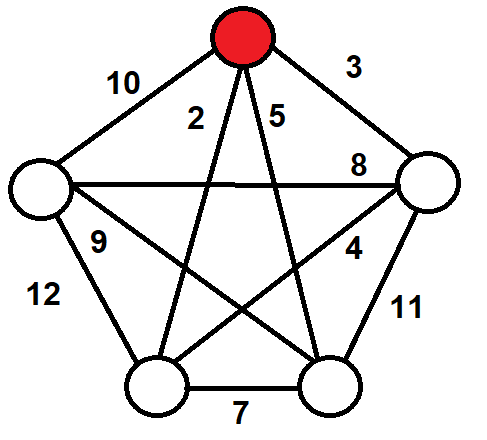
\includegraphics[scale=0.5]{Przyklad2}
        \centering
        \caption{Problem komiwojażera (Travelling Salesman Problem, TSP). Na rysunku pomocniczym liczby symbolizują wagi krawędzi. Węzeł oznaczony
        kolorem czerwonym odpowiada węzłowi startowemu, do którego należy wrócić. Długości krawędzi nie zachowują wskazanych przez wagi proporcji.}
        \label{TSP}
    \end{figure}
    Problem komiwojażera jest popularnym zagadnieniem optymalizacyjnym, którego istotą jest wskazanie ścieżki o najmniejszej sumie wag krawędzi, 
    która przechodzi dokładnie jeden raz przez każdy wierzchołek i wraca do wierzchołka startowego. Często problem wędrującego 
    komiwojażera przedstawiany jest przy pomocy kuriera oraz domów, które musi odwiedzić (za wierzchołek startowy uważa się magazyn,
    w którym kurier rozpoczyna swoją pracę). Mimo faktu, iż w przykładzie \ref{TSP} występuje jedynie 5 miejsc, 
    w których musi zatrzymać się kurier, utworzenie optymalnego planu dla przedstawionej sytuacji jest nielada wyzwaniem. Z tego powodu 
    ludzie postanowili skorzystać z potężnych mocy obliczeniowych komputerów przy generowaniu bardziej skomplikowanych planów.


\section{Planowanie przy użyciu komputerów}

    \subsection{STRIPS}
    \label{STRIPSRozdział}
    W 1971 roku Panowie: Richard Fikes oraz Nils Nillson z Standford Research Institute (SRI International, 
    jeden z najsłynniejszych na świecie ośrodków badawczych) zdecydowali się na przedstawienie światu
    nowego podejścia w dziedzinie planowania o nazwie \textbf{STRIPS} (\textbf{ST}anford \textbf{R}esearch \textbf{I}nstitute
    \textbf{P}roblem \textbf{S}olver)\cite{STRIPS}.
    \textbf{STRIPS} rozwiązuje wskazany problem poprzez przeszukiwanie wszystkich stanów świata, aż do momentu
    gdy znajdzie taki, w którym wskazane cele są spełnione. Ważnym założeniem programu jest istnienie
    ciągu akcji, który gwarantuje otrzymanie celu. Zadanie to jest realizowane poprzez znalezienie
    sekwencji operatorów, która konwertuje wymodelowany stan początkowy, w model, w którym wszystkie 
    zdefiniowane cele są spełnione. Defnicje operatorów, stanu początkowego oraz celu są niemalże identyczne jak 
    \ref{StanyPoczatkowe}, \ref{Akcje} i \ref{Cel}, z tym, że definicja Akcji została w naturalny sposób rozwinięta o ciąg przyczynowo-skutkowy. Zauważono, iż w skład każdej akcji 
    poza samą czynnością wchodzą dwie składowe, nazywane środowiskowymi- warunki zajścia oraz efekty zajścia. 
    \begin{definition}
        \label{WarunekAkcji}
        \textbf{Warunkiem}- zajścia akcji jest istnienie odpowiedniej konfiguracji świata, dzięki której akcja może zostać wykonana.
    \end{definition}
    \begin{definition}
        \label{EfektAkcji}
        \textbf{Efektem}- zajścia akcji są zmiany, które zaszły w przedstawionym świecie ze względu na jej wykonanie.
    \end{definition}
    Mówiąc kolokwialnie, każda akcja ma swoją przyczynę oraz swój skutek. \textbf{Przyczyną} akcji w przykładzie \ref{Przyklad1} jest znajdowanie się klocka na lewej platformie. Gdyby
    klocek A znajdował się na prawej platformie, wykonanie akcji przesunięcia klocka z platformy lewej na prawą nie mogłoby zostać wykonane, natomiastem \textbf{efektem} akcji jest 
    przeniesienie klocka na prawą platformę. Łatwo zauważyć, iż brak innych obiektów na platformie prawej jest niezbędny, aby klocek mógł zostać tam przeniesiony.
    Kolejną naturalną obserwacją jest stwierdzenie, iż przeprowadzenie akcji dodaje nam nowe informacje o świecie w dwóch kontekstach:
    \begin{itemize}
        \item Dodającym- pojawienie się lub podtrzymanie danej składowej świata
        \item Usuwającym- pozbawienie świata danej składowej
    \end{itemize}
    Po wykonaniu czynności z przykładu \ref{Przyklad1} wyróżniamy trzy typy nowych informacji:
    \begin{itemize}
        \item Warunek- Obecnośc klocka na lewej platformie, prawa platforma jest pusta
        \item Efekt dodający- Obecność klocka na prawej platformie
        \item Efekt usuwający - Platforma lewa jest pusta
    \end{itemize}
    W rozważanym podejściu każda z czynności zdefiniowana jest przy pomocy wyżej wskazanych trzech składowych.

        Takie zdefiniowane świata okazuje się wystarczające do rozwiązywania problemów pokroju rearanżacji obiektów czy 
    nawigowania w ściśle zdefiniowanej przestrzeni, czego najlepszym przykładem, jest pierwszy robot do realizacji ów zadań- \textbf{Shakey}.
    Shakey był pierwszym robotem, który dzięki zainstalowanemu oprogramowaniu,
    posiadał umiejętność analizy własnego otoczenia. Dzięki zaimplementowanemu podejściu 
    STRIPS (oczywiście z odpowiednimi dostosowaniami do sytuacji) był w stanie rozwiązywać problemy z zakresu wyznaczania drogi,
    czy planowania rozmieszczenia obiektów w pokojach.
    Ze względu na swoją innowacyjność i przełomowość często jest nazywany archetypem
    dzisiejszych autonomicznych samochód czy militarnych dronów.

    Dzięki swojej roli w rozwoju planowania z użyciem komputerów, STRIPS został dodatkowo wyróżniony- od jego nazwy pochodzi języki opisu świata korzystający
    z trójki: stan początkowy, akcja oraz cel. Przez następne lata rozwiązania w obszarze planowania silnie bazowały na wprowadzonym w powyższej pracy opisie świata.

    \subsection{Rozwiązywanie ludzkich problemów}
    W 1972 roku Panowie Allen Newell i Herbet Simon opublikowali książkę pod nazwą \textbf{Human Problem Solving}, której tłumaczenie
    znajduje się w tytule opisywanej sekcji. Założenie odnośnie otrzymywanych przez algorytm rozwiązujący problem danych 
    pozostało zgodne z opisem w sekcji \ref{STRIPSRozdział}, jednakże autorzy pracy zauważyli, iż utworzony w ten sposób 
    obszar działań (\textit{problem space}) może osiągać niebotyczne rozmiary. Chcąc odpowiedzieć na pytanie, 
    w jaki sposób ludzie wybierają odpowiednie operacje w danej sytuacji, zauważyli, iż ludzie często wykorzystują \textit{skróty},
    które wynikają bezpośrednio z intuicji. Człowiek ze względu na swoją naturę będzie dążył do zużycia jak najmniejszych 
    pokładów energii w celu osiągnięcia wyznaczonego celu. Na tej podstawie rozpoczęło się formowanie 
    technik rozwiązywania problemów zwanych \textbf{heurystykami}. Początkowe heurtystki ograniczały się do zastosowania 
    pewnych ograniczeń jeśli chodzi o wyznaczanie zbioru operatorów, na przykład poprzez unikanie powtórzeń (\textit{repeat-state avoidance})
    oraz unikanie powrotów do stanó już znanych (\textit{backup avoidance}). Na przestrzeni następnych lat pojęcie heurystyki rozwinie się diametralnie, jednakże
    zachowa swoją pierwotną definicję szukania rozwiązań na skróty lub kolokwialnie mówiąc \textit{na ludzkie oko}.  

    \subsection{Liniowy i częściowy porządek}
    Na początku lat 70 ubiegłego wieku do tworzenia prostych planów wykorzystywano również pojęcie 
    liniowego porządku (\textit{total order}) sekwencji akcji. W tym podejściu, ochrzonym mianem \textbf{planowanie liniowe}
    (\textit{linear planning}) dla każdego z celów  próbowano utworzyć odpowiedni podplan, który go osiągał.
    Następnie ów plan łączono przy pomocy odpowiedniego porządku akcji w jeden spójny plan.
    Ze względu na wady tego podejścia, jak długi czas formowania planu oraz możliwość wystąpienia konfliktów między 
    odpowiednimi celami planu, co na początku nie było takie oczywiste, zamiast liniowego porządku zaczęto wykorzystywać porządek częściowy (\textit{partial order}),
    którego przykładem jest omawiany \textbf{GRAPHPLAN}.







    \subsection{ADL i PDDL}
    Action Description Language (w skrócie \textbf{ADL}) zostało zaproponowane przez pana Edwina Pednault'a  w 1987 roku jako usprawnienie 
    języku opisu STRIPS. Ów system automatycznego planowania został zaprojektowany z myślą o przyszłej implementajci w nowoczesnych na tamten czas robotach.
    Główną ideą stojącą za utworzeniem tego języka opisu problemów było zauważenie, iż język STRIPS nie potrafi poradzić sobie z sytuacjami, gdy
    powstanie danego efektu jest niedeterministyczne. Dodatkowym aspektem, które wprowadzenie znacznie poprawiło wydajność metodologii ADL względem STRIPS 
    było wykorzystanie zasady \textbf{otwartego świata}, która mówi, iż rzeczy nieokreślone w świecie są uznawane jako \textit{nieznane}, a nie jako 
    fałszywe, jak to było w STRIPS (\textbf{zasada zamkniętego świata}). Dodatkowo, 

    Planning Domain Definition Language (w skrócie \textbf{PDDL}) 

    \subsection{Nowoczesne rozwiązania}
    TO-DO
    
    Między powstaniem metodologii STRIPS a jej rozszerzeniami w postaci ADL lub PDDL powstawały również inne podejścia, w tym silnie 
    bazujący na grafach i ich możliwościach algorytm o wdzięcznej nazwie \textbf{GRAPHPLAN}.







	\cleardoublepage

	\chapter{GRAPHPLAN}
\thispagestyle{chapterBeginStyle}

\section{Wprowadzenie}
    \textbf{GRAPHPLAN} jest algorytmem do planowania akcji działający w dziedzinie zdefiniowanej
    przez język STRIPS, dodatkowo bazuje na paradygmacie, który autorzy algorytmu określają jako "graf planujący" \cite{GRAPHPLAN}.
    \begin{figure}[H]
        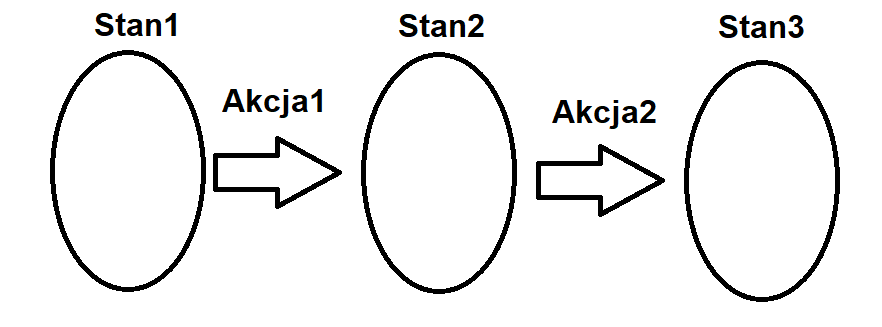
\includegraphics[scale=0.5]{PlanningGraph}
        \centering
        \caption{Najogólniejsza forma grafu planującego. Składa się on z węzłów, zwanych stanami oraz krawędzi zwanych akcjami. Docelowo poszczególne 
        stany oraz akcje są parami różne, jednak mogą zajść sytuacje, gdy powtórzenie któregoś z komponentów będzie wymagane do uzyskania odpowiedniego
        celu.}
        \label{PlanningGraph}
    \end{figure}
    Pierwotną ideę grafu planującego przedstawiono na obrazku \ref{PlanningGraph}. W trakcie dalszego omawiania metodologii GRAPHPLAN powyższa 
    rycina będzie pojawiała się ponownie z coraz to większym poziomiem szczegółowości.
    Ze względu na fakt, iż Graphplan opiera się na języku STRIPS musi mieć jasno zdefiniowane: stan początkowy, akcje oraz cel, który pragniemy uzyskać.
    Dzięki swojej strukturze Graphplan w swojej naturze podobny jest do programowania dynamicznego.

\section{Warunki początkowe}
    \label{RozdzialWarunkiPoczatkowe}
    \begin{definition}
        \label{ZasadaSwiata}
        \textbf{Zasada zamkniętego świata} - Zasada, wedle której pojęcia, które nie są ściśle opisane w świecie są nieprawdziwe.
    \end{definition}
    GRAPHPLAN, w odróżnieniu od człowieka, musi być w posiadaniu całej wiedzy o świecie, aby móc rozpocząć działanie. Przez całą wiedzę o świecie rozumie się
    posiadanie informacji na temat każdego obiektu oraz jego stanu. Wiąże się to ściśle z faktem,
    iż GRAPHPLAN operuje zgodnie z definicją \ref{ZasadaSwiata}. 
    Przed dalszą częścią pracy należy dokonać pewnego wyróżnienia. Słowo \textbf{stan} pojawia się w dwóch znaczeniach:
    stan jako pojedyncza informacja o obiekcie w świecie (Przykład: klocek B na stole numer 3) oraz stan, jako zbiór wszystkich takich informacji w danym momencie czasu.
    Z tego względu wprowadzono nowe pojęcie- "Poziom stanów", które należy stosować jako oznaczenie wszystkich informacji o świecie w danym momencie.
    \begin{definition}
        \label{PoziomStanow}
        \textbf{Poziom stanów} - Zbiór informacji o stanach wszystkich obiektów w świecie w danej jednostce czasu \textit{t}
    \end{definition}
    Szczególnym poziomem stanów jest poziom oznaczany jako pierwszy i nazywany \textbf{Warunkami początkowymi}, którego poprawne zdefiniowanie jest kluczowym aspektem w kontekscie
    uzyskania poprawnego wyniku przez algorytm.
    Analizując ponownie przykład \ref{Przyklad1} mylnym jest myśleć, iż jedyną informacją, jaką algorytm powinien posiadać o świecie jest pobyt klocka A na lewej platformie. Również
    istotną informacją jest brak klocka na platformie prawej, czyli informacja, ze jest on \textit{pusty}. Mimo poczucia nadmiarowości tej informacji, w dalszej części pracy wyjaśni
    się, dlaczego ta informacja jest niezbędna do uzyskania poprawnego wyniku.
    Przykład świata przedstawionego oraz skonstruowanego dla niego stanu początkowego:
    \begin{figure}[H]
        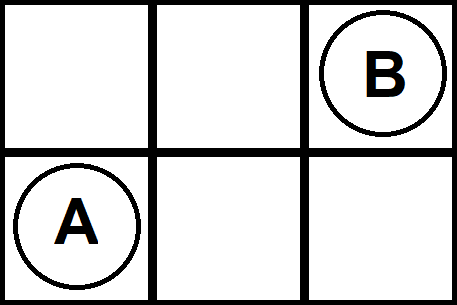
\includegraphics[scale=0.5]{PrzykladSP}
        \centering
        \caption{Przykładowy moment startowy przyszłego planu. Za pomocą okręgów oznaczono roboty, natomiast poprzez kwadraty oznaczone są kafelki- miejsca,
        po których mogą poruszać się roboty.}
        \label{PrzykladSP}
    \end{figure}
    Na powyższym przkładzie, zgodnie z ideą Graphplanu wyszczególniamy 6 stanów początkowych. Dodatkowo należy doprecyzować pojęcie bycia robota na danym kafelku. Wykonano to 
    przy pomocy dwuargumentowej relacji \textit{na}, która jako pierwszy argument przyjmuje sygnaturę robota, a na drugim- numer kafelka. Na potrzeby przykładu ustalono, iż 
    numerowanie odbywa się rzędami od lewej do prawej. Zgodnie z tymi ustaleniami pozycję robotów A i B możemy określić w następujący sposób: \textit{$na(A,4)$} oraz 
    \textit{$na(B,3)$}. Również pustość kafelków należy sformalizować wprowadzając relację jednoargumentową o nazwie \textit{pusty}, która przyjmuje jako argument numer
    pustego kafelka. Reasumując, zbiorem stanów początkowy dla analizowanego przykładu \ref{PrzykladSP} jest: 
    \begin{equation}
        \{pusty(1),pusty(2),na(B,3),na(A,4),pusty(5),pusty(6)\}
        \label{ZbiorPoczatkowy}
    \end{equation}
\section{Akcje}
    \label{RozdzialAkcje}
    Posiadając dobrze określony stan początkowy następnym krokiem będzie zdefiniowanie akcji. Zgodnie z \ref{Akcje} oraz wzmiance o akcjach w planerze STRIPS,
    akcja musi składać się z trzech komponentów:
    \begin{itemize}
        \item Czynności
        \item Warunków zajścia
        \item Efektów zajścia
    \end{itemize}
    Z tego powodu każdą z akcji będziemy traktować jako trójkę 
    \begin{equation}
        A=(C,W,E)
    \end{equation}
    gdzie każda z liter odpowiada pierwszej literze wyżej wymienionego pojęcia. 
    W skład efektów wchodzą dwa pojęcia wprost z terminologii STRIPS- dodające i usuwające. Dzięki takiemu podziałowi łatwiejszym będzie 
    zachowanie silnego podziału między przyczynami a efektami akcji. 
    Jedyną czynnością, którą należy brać pod uwagę w ramach \ref{PrzykladSP} jest czynność \textit{ruch}, którą definiujemy jako trzyargumentową relację:
    \begin{equation}
        ruch(R,S,D)
    \end{equation}
    , gdzie R odpowiada robotowi, który musi się przemieścić z kafelka oznaczonego literą S (kafelek startowy) na kafelek oznaczony
    literą D (kafelek docelowy).
    
    Następnymi składowymi są odpowiednio \textit{Warunki} jak i \textit{Efekty}. Warunki traktujemy jako zbiór wszystkich stanów, które muszą być 
    prawdziwe w danej jednostce czasu. Jeśli choć jeden stan nie jest spełnialny, opisywana akcja nie może zostać wykonana w danym ruchu.
    Efekty natomiast definiujemy jako następującą parę:
    \begin{equation}
        E=(D,U)
    \end{equation}
    gdzie D oznacza efekty dodające, a U- efekty usuwające.
    \begin{figure}[H]
        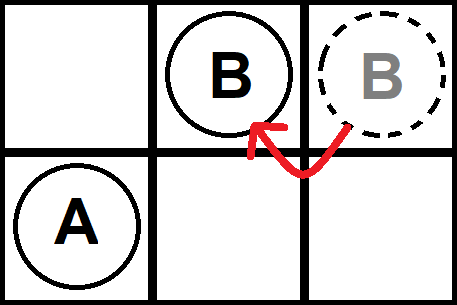
\includegraphics[scale=0.5]{PrzykladRuch}
        \centering
        \caption{Obrazowe przedstawienie ruchu robota B z kafelka 3 na kafelek 2}
        \label{PrzykladRuch}
    \end{figure}
    Niech rozpatrywaną akcją będzie przemieszczenie robota B z pozycji 3 na pozycję 2,
    przedstawiona na \ref{PrzykladRuch}. Biorąc pod uwagę, iż stanem początkowym jest \ref{ZbiorPoczatkowy} Warunkami zajścia zdarzenia
    będą: $na(R,S)$ oraz $pusty(D)$. Dla efektów natomiast sytuacja wygląda następująco: efektami dodającymi są $na(R,D)$ oraz $pusty(S)$, które informują o tym, iż klocek 
    wykonał ruch z kafelka S na kafelek D, a efektami usuwającymi $\sim na(R,S)$ oraz $\sim pusty(D)$, które informują o tym, iż kafelek S został zwolniony, 
    oraz robot nie znajduje się już na kafelku S. Przy pomocy matematycznego symbolu negacji wyrażono nieprawdziwość danego stanu. Ze względów estetycznych 
    oraz ułatwiających analizowanie pracy negacje stanów w dalszej części pracy wyrażono również przy pomocy polskiej partykuły przeczącej \textbf{nie}. 
    Dla przykładu pojęcia $\sim pusty(1)$ oraz $niepusty(1)$ z perpsektywy wprowadzonej terminologii są tożsame. 

        Posiadająć następującą wiedzę poniżej zdefiniowano jedyną akcję znajdująca się w prezentowanym przykładzie:
    \begin{equation}
        \label{Ruch}
        A=(ruch(R,S,D),\{na(R,S),pusty(D)\},\{na(R,D),pusty(S),\sim na(R,S),\sim pusty(D)\})
    \end{equation}
    Podstawiając za $R=B$, $S=3$, a $D=2$ otrzymujemy następującą akcję:
    \begin{equation}
        A=(ruch(B,3,2),\{na(B,3),pusty(2)\},\{na(B,2),pusty(3),\sim na(B,3),\sim pusty(2)\})
    \end{equation}
    
    Analogicznie można zdefiniować ruch na kafelek numer 6, oraz dwa ruchy dla robota o sygnaturze A.


    \subsection{Typy akcji}
    Definicja \ref{ZasadaSwiata} znajduje również swoje odzwierciedlenie w akcjach. Niech rozpatrywanym przykładem będzie wciąż przykład \ref{PrzykladSP}.
    W pierwszym kroku wykonano akcję $ruch(B,3,2)$.Z persepktywy człowieka jest to wystarczająca informacja, aby móc wydedukować, co we wskazanym etapie
    generowania planu  dzieje się z robotem \textbf{A}. Otóż robot A w pierwszym ruchu zostaje na tym samym kafelku. 
    Jednakże ze względu na zamkniętość świata 
    algorytmu należy go również poinformować go o tym, w jakim stanie po pierwszym kroku ma znajdować się robot A. Wykonywane jest to przy pomocy 
    akcji, zwanych \textbf{akcjami potrzymującymi}.
    \begin{definition}
        \label{Persist}
        \textbf{Akcja podtrzymująca} - Akcja, która przenosi stan obiektu w czasie $t$ nienaruszonym do poziomu stanów w czasie $t+1$
    \end{definition}
    Akcjami podtrzymującymi należy również informować świat o stanach kafelków, które nie brały udziału w akcji robota B. Przykładem takiego jest 
    kafelek 1, który w stanie początkowym, jak i w stanie następnym ciągle zachowuje swój stan jako pusty. Akcje podtrzymujące oznaczono 
    słowem kluczowym \textbf{zostań}
    Ponadto akcja typu \textit{ruch}, które aktywnie zmienia stan świata w dalszej części pracy otrzyma miano \textbf{akcji aktywnej}.
    \begin{definition}
        \label{Active}
        \textbf{Akcja aktywa} - Akcja, która zmienia stan obiektu między stanami w czasie $t$ i $t+1$.
    \end{definition}

    Posiadając powyższy podział akcji poniżej przedstawiono pełen zbiór akcji w pierwszym kroku algorytmu. Wartym odnotowania jest, iż ze względów
    estetycznych podawawnie akcji podtrzymujących będzie często pomijane, jednakże nie można zapomnieć o ich występowaniu oraz o ich kluczowej roli 
    w generowaniu precyzyjnego planu.
    \begin{align*}
        Akcje &= \{zostan(pusty(1)),zostan(pusty(2)),zostan(pusty(5)),zostan(pusty(6)),zostan(na(B,3)), \\
        &zostan(na(A,4)),ruch(B,3,2),ruch(B,3,6),
        ruch(A,4,1),ruch(A,4,5)\}
    \end{align*}
    Należy również nadmienić, iż podobnie jak w stanach, dla akcji wprowadza się pojęcie \textbf{Stanu akcji}, które funkcjonuje jako zbiór 
    składający się ze wszystkich możliwych akcji do wykonania w danej jednostce czasu.
    \begin{figure}[H]
        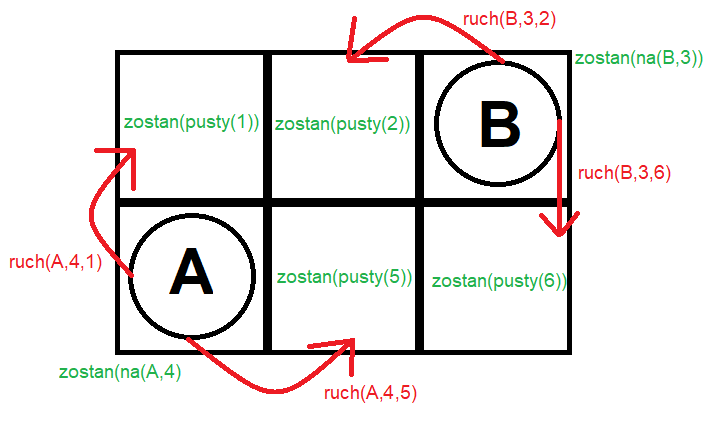
\includegraphics[scale=0.5]{PrzykladAkcje}
        \centering
        \caption{Obrazowe przedstawienie wszystkich akcji w pierwszym kroku algorytmu, akcje opisane przy użyciu czcionki o kolorze zielonym 
        symbolizują akcje podtrzymujące, natomiast o kolorze czerwonym- akcje aktywne}
        \label{PrzykladAkcje}
    \end{figure}
    

\section{Definiowanie świata}
    Zdecydowanie najtrudniejszym aspektem modelowania świata jest dokładne przedstawienie wszystkich zależności, jakie algorytm musi znać,
    aby mógł bezbłędnie wnioskować w prezentowanej przestrzeni. Analizując przykład \ref{PrzykladSP} dokonano przedstawienia schematu 
    generowania poziomu stanów początkowych oraz poziomu akcji. Zadając pytanie algorytmowi \textit{Jakie działania należy podjąć, aby jak najszybciej
    przesunąć robota A z klocka 4 na klocek 6} algorytm odpowie w następujący sposób: $ruch(A,4,6)$, jednakże przyglądając się uważnie przedstawionemu światu 
    zauważono, iż taki plan byłby realny jedynie, gdyby akcja $ruch$ oznaczała latanie- wtedy faktem jest, iż istnieje możliwość pominięcia kafelka 5 podczas 
    przemieszczenia. Niespójnośc ta pojawiła się z faktu, iż w żadnym momencie nie określono w jaki sposób dokładnie funkcjonuje czynnośc oznaczona jako \textit{ruch}.
    Wedle definicji \ref{Ruch} wszystkie warunki, aby robot mógł przemieścić się z kafelka 4 na 6 zostały spełnione.

    Naprawić ten problem można przy pomocy uściślenia wykonywanej czynności. Do tego potrzebne będzie wprowadzenie relacji \textit{sąsiad}, która 
    przyjmuje dwa argumenty- numery kafelków, które ze sobą sąsiadują. Zakładając, iż sąsiadujące kafelki to takie, które mają wspólną ścianę, sąsiadami 
    kafelka 1 są kafelki: 2 oraz 4. Dla pozostałych przestrzeni dokonano analogicznego wygenerowania listy sąsiadów. Dzięki tej operacji, 
    akcję ruch zdefiniowano w następujący sposób:
    \begin{equation}
        ruch(R,S,D) \textnormal{:-} sasiad(S,D)
    \end{equation}
    Czynność ruchu w powyższym przypadku została określona zgodnie z semantyką języka programowania \textbf{PROLOG}. Należy to rozumieć w następujący sposób:
    po lewej stronie znaku \textbf{:-} znajduje się \textit{konkluzja}, natomiast po prawej- \textit{przesłanka}. Naturalnym odczytem przedstawionej sytuacji
    będzie zdanie \textit{"Jeśli kafelki S i D są sąsiadami to możliwym do wykonania jest ruch między tymi kafelkami"}
    \begin{figure}[H]
        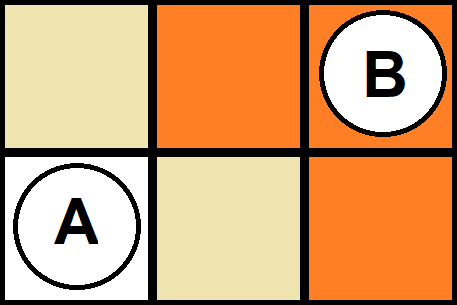
\includegraphics[scale=0.5]{PrzykladSasiad}
        \centering
        \caption{Graficzne przedstawienie relacji sąsiedztwa dla kafelka numer 4. Kolorem kremowym oznaczono miejsca, z którymi sąsiaduje, natomiast 
        pomarańczowym- te, z którymi nie sąsiaduje. Oznacza to, iż do kafelków pomarańczowych nie można dostać się wykonując jeden ruch}
        \label{PrzykladAkcje}
    \end{figure}
    Taka definicja ruchu pozwala w skuteczny sposób oddać intuicję, która wynika z poglądowego obrazka przedstawiającego rozpatrywany świat.
    Niewystarczającym jest określenie relacji $sasiad(1,2)$, gdyż wedle tego faktu kafelek pierwszy sąsiaduje z kafelkiem drugim, jednakże nie oznacza 
    to, iż kafelek drugi sąsiaduje z kafelkiem pierwszym. Z tego dla każdej pary kafelków A i B do zbioru sąsiadów należy dodać dwie relacje:
    $sasiad(A,B)$ oraz $sasiad(B,A)$. Inna sytuacja byłaby, gdyby ruch był możliwy jedynie w jedną stronę, jednakże tutaj taki stan rzeczy nie występuje.


    Oprócz definicji sąsiedztwa należy również zabezpieczyć się przed sytuacją, gdy dwa roboty będą chciały w tym samym momencie znaleźć się na tym samym 
    kafelku. Dodatkowo kafelek A nie może znajdować się w dwóch stanach jednocześnie: $pusty(A)$ oraz $na(R,A)$, gdzie R oznacza dowolnego robota. 
    Wymodelowanie tych ograniczeń jest prostym, lecz istotnym zadaniem implementując przedstawianą metodologię, które zostanie poruszone w ramach 
    przedstawiania pojęcia "wzajemnego wykluczania".
    
    
    Odpowiednie wymodelowanie świata wedle wzorców języka STRIPS może wydawać się trudnym oraz żmudnym zajęciem, jednakże przebrnąwszy 
    przez ten etap algorytm jest zwarty i gotowy do generowania planów dla wprowadzonych celów.


\section{Warstwy grafu}
    Składowe planu grafującego można podzielić na dwa typy: jeden, wyszczególniony jako poziomy stanów oraz drugi- poziomy akcji. Aby lepiej 
    uwidocznić zależność poziomu akcji od warunków początkowych oraz zależność kolejnego poziomu stanów od efektów akcji graf planujący 
    z \ref{PlanningGraph} ulegnie lekkiej modyfikacji. 
    \begin{figure}[H]
        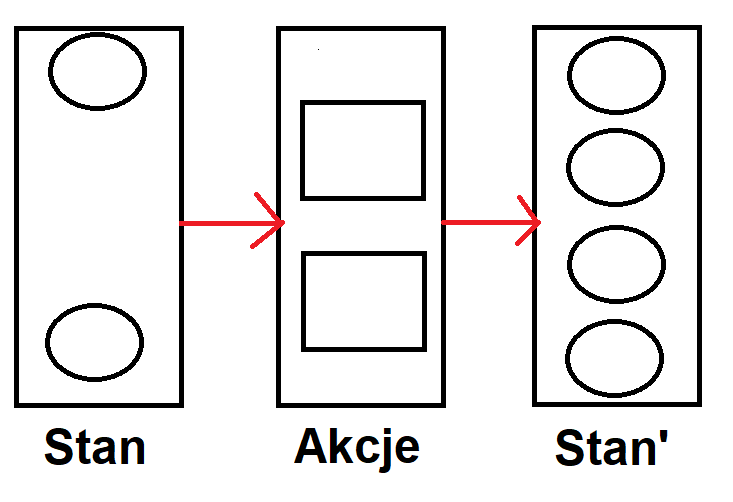
\includegraphics[scale=0.5]{PlanningGraphStates}
        \centering
        \caption{Modyfikacja do grafu planującego wprowadzona w poprzednich podrozdziałach. Wprowadzono zależności akcji od stanu poprzedniego, oraz stanu 
        następnego od akcji.}
        \label{PlanningGraphStates}
    \end{figure}
    Następnym krokiem będzie wprowadzenie definicji \textbf{Warstwy grafu}
    \begin{definition}
        \label{Warstwa}
        \textbf{Warstwą} - grafu nazywamy połączenie poziomu stanów oraz wynikającego z niego poziomu akcji
    \end{definition}
    Przez $i$-tą warstwę grafu oznaczono stan świata w $i$-tym momencie czasu. Ze względu na charakterystykę planera czas traktowany jest w sposób dyskretny-
    każda ze zdefiniowanych akcji zajmuje zawsze tyle samo czasu oraz zawsze kończy się tym samym efektem. Poziomy stanów jak i poziomy akcji 
    należące do tej samej $i$-tej warstwy nazywamy poprzez dołączenie do ich nazwy numera, odpowiadającego obecnej iteracji algorytmu
    iteracji algorytmu.
    \begin{figure}[H]
        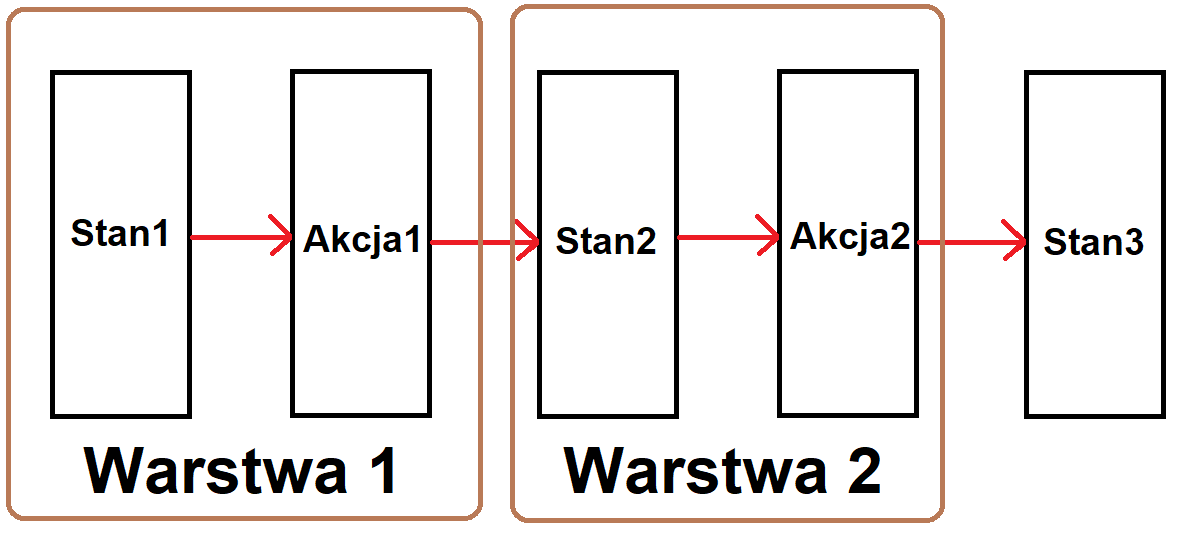
\includegraphics[scale=0.5]{PlanningGraphLevels}
        \centering
        \caption{Przedstawienie sposobu wyznaczania warstw w algorytmie planującym. Poziom stanów oraz akcji wchodzący w skład danej warstwy 
        wyróżniony jest poprzez konkatenację nazwy oraz liczby symbolizującej numer warstwy.}
        \label{PlanningGraphLevels}
    \end{figure}
    Dzięki wprowadzeniu definicji warstwy po wygenerowaniu 
    planu natychmiast wiadomo ile kroków należy wykonać, a co za tym idzie- ile czasu należy poświęcić, aby osiągnąć ustalony cel. 

    \section{Równoległość}
    \label{Rownoleglosc}
    W poprzednich paragrafach na pojedynczym poziomie akcji rozpatrywano conajwyżej jedną akcję aktywną, jednakże główną siła GRAPHPLANU, jest 
    możliwość jego reprezentacji jako częściowego porządku. To pozwala w prosty sposób wprowadzić pojęcie równoległości między akcjami. 
    \begin{definition}
        \label{Warstwa}
        Dwie (lub więcej) akcje  mogą zostać wykonane \textbf{równolegle}, gdy po ich wykonaniu w tej samej warstwie $i$, warstwa $i+1$ nie będzie 
        zawierała w sobie żadnych sprzeczności.
    \end{definition}
    Przyglądając się rysunkowi \ref{PrzykladSP} od razu należy zauważyć, iż w stanie początkowym ruch robota A nie wpływa w żaden sposób na otoczenie
    robota B. Z tego względu dwie przykładowe akcje $ruch(A,4,5)$ oraz $ruch(B,3,2)$ wręcz należy wykonać w tej samej jednostce czasu, czyli w pierwszym
    poziomie akcji. 
    \begin{figure}[H]
        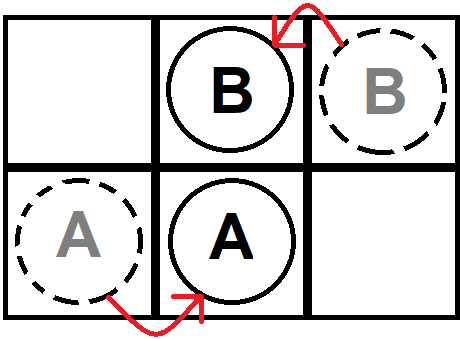
\includegraphics[scale=0.5]{PrzykladRownolegle}
        \centering
        \caption{Przykład możliwości zastosowania równoległości w planowaniu działania. Należy zauważyć, iż ruchy robotów w żaden sposób ze sobą
        nie kolidują.}
        \label{PrzykladRownolegle}
    \end{figure}
    
    Po wprowadzeniu definicji równoległości, również definicja kroku musi ulec ewolucji. 
    \begin{definition}
        \label{Krok}
        \textbf{Krokiem} algorytmu nazywamy zbiór wszystkich możliwych do realizacji akcji w danej warstwie.
    \end{definition}
    Dzięki naniesionej poprawce pozbywamy się łatki mówiącej o tym, iż pojedyncza zmiana stanu jest ściśle związana z jedną akcją.W tym miejscu należy 
    zauważyć, iż poprzednie analizy zawierały spore uproszczenie, gdyż akcje podtrzymujące również należą do kroku algorytmu, co zostało zaprezentowane
    w trakcie kreowania pierwszej warstwy akcji dla rozpatrywanego przykładu. 

    Istnieją przypadki, gdy podmiot realizujący plan nie jest w stanie wykorzystać benefitów płynących z możliwości dokonywania akcji równolegle, 
    na przykład ze względu na ograniczone zasoby. GRAPHPLAN również rozwiązuje ten problem, pozwalając przekształcać swój częsciowy porządek 
    na porządek liniowy w dość dowolny sposób. Otóż akcje z danej warstwy mogą być wykonywane w dowolnej kolejności, gdyż w żaden sposób ze sobą nie 
    kolidują. Z persepktywy algorytmu najważniejszym jest, aby stan świata $i$ i $i+1$ był zgodny z informacjami jakie posiada o świecie. Zgodnie z
    przykładem \ref{PrzykladRownolegle} widać, iż to, czy akcja $ruch(A,4,5)$ zostanie wykonana przed akcją $ruch(B,3,2)$ lub to, czy akcja 
    $ruch(B,3,2)$ odbędzie się prxed $ruch(A,4,5)$- efekt końcowy jest identyczny.

    \subsection{Wzajemne wykluczanie}
    Twórcy algorytmy wprowadzając równoleglość, zdawali sobie sprawę z mocy tego podejścia. Dzięki temu ogromna liczba planów ulega redukcji
    jeśli chodzi o wymagany czas wykonania. Jednakże równoległość wprowadza kolejny istotny problem w prezentowanym świecie, a mianowicie- co, gdy
    wykonanie dwóch akcji będzie wprowadzało sprzeczność w następnym poziomie świata? Sytuacja ta została przedstawiona na poniższym rysunku
    \begin{figure}[H]
        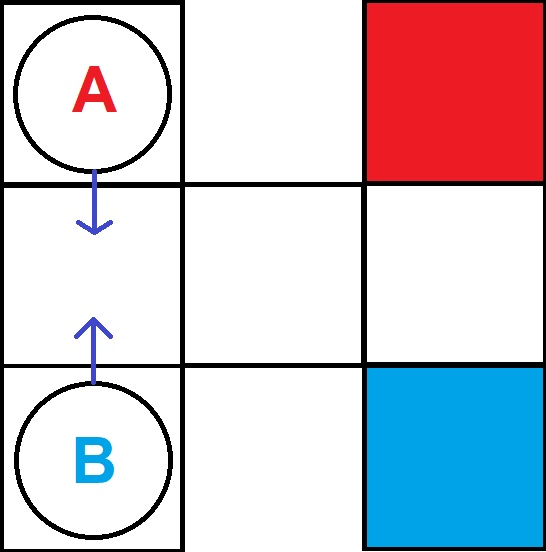
\includegraphics[scale=0.5]{PrzykladRownolegleZle}
        \centering
        \caption{Przykład świata, w którym wprowadzenie równoległości dla pierwszej warstwy algorytmu jest niemożliwe. 
        Dwa roboty próbują przejść na ten sam kafelek
        w tej samej jednostce czasu, co z perspektywy kafelka powoduje konflikt. Odpowiednio kolorami:
        czerwnoym i niebieskim oznaczono roboty, oraz kafelki, które są ich celem.}
        \label{PrzykladRownolegle}
    \end{figure}
    
    Zmusiło to twórców algorytmu do wporwadzenia pojęcia \textbf{relacji wykluczania}. 
    O akcjach wzajemnie się wykluczających (ang. actions mutually exclusive, \textbf{mutex}) wspomiano w ramach definiowana świata. Pojęcie ów można 
    określić w następujący sposób:
    \begin{definition}
        \label{Warstwa}
        \textbf{Relacją wzajemnie wykluczającą się} - jest relacją między akcjami(stanami), która informuje o tym, iż nie istnieje plan taki,
        aby dwie wybrane akcje(stany) mogły być prawdziwe w tej samej jednostce czasu $t$
    \end{definition}
    Przykładem stanów wykluczających jest para: $pusty(1)$ oraz $\sim pusty(1)$. Kafelek nie może być pusty jak i niepusty jednocześnie.
    Przykład dwóch akcji wykluczających przedstawiono na rysunku \ref{PrzykladRownolegle}. Należy zauważyć, iż wzajemne wykluczanie się 
    jest rozpatrywane warstwowo.
    Kolejnym naturalnym krokiem jest ustalenie, kiedy akcje oraz stany są ze sobą w relacji wykluczającej. 

    \subsubsection{Wykluczanie się stanów}
    Dwa stany są ze sobą w relacji wzajemnie wykluczającej w dwóch następujacych przypadkach:
    \begin{enumerate}
        \item Negacja- przypadek, w którym jeden ze stanów jest negacją drugiego
        \item Niespójne powstanie- wszystkie akcje z poprzedniej warstwy, które prowadza 
        do utworzenia ów stanów są ze sobą parami w relacji wykluczającej
    \end{enumerate}
    Ze względu na naturalność pojęcia negacji zbędnym jest wprowadzenie większego przykładu niż przedstawienie, iż dla każdego obiektu istnieje 
    para stanów znajdujących się w relacji wykluczającej. Niech za przykład posłuży pustość kafelka. Kafelek nie może być jednocześnie pusty, jak 
    i niepusty, co sprowadza się, iż stan $pusty(kafelek)$ jak i $\sim pusty(kafelek)$ są niemożliwe do zawarcia w jednej warstwie planu.

    Dla kontrastu przedstawienie przypadku, w którym zachodzi \textbf{niespójne powstawanie} jest trudniejsze i wymaga użycia 
    przykładowej ilustracji:

    \begin{figure}[H]
        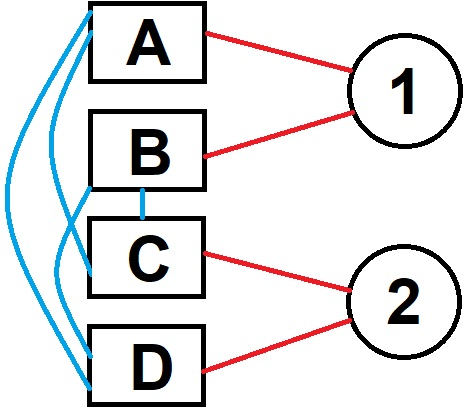
\includegraphics[scale=0.5]{PrzykladWykluczenie3}
        \centering
        \caption{Urywek planu przedstawiający sytuację, w której dwa stany powstają w sposób niespójny. Zgodnie z założeniami akcje oznaczone są przy 
        pomocy prostokątów, stany- okręgów, miedzy akcjami a stanami czerwone linie symbolizują które stany są efektami których akcji, natomiast linie
        niebieskie między akcjami symbolizują powstałe między nimi \textit{mutexy}}
        \label{PrzykladWykluczenie3}
    \end{figure}

    Zgodnie z nienaturalnym przykładem \ref{PrzykladWykluczenie3} należy zauważyć, iż stany 1 oraz 2 nie mogą 
    znajdować się jednocześnie w planie ze względu na to, iż każda z akcji, która generuje stan 1 (B,C) znajduje się w relacji 
    wzajemnie wykluczającej z każdą akcją, która generuje stan 2 (C,D). Oznacza to, iż ów dwa stany powstają w sposób \textbf{niespójny}.
    
    Z reguły ten typ wykluczeń występuje po większej liczbie kroków dla bardziej rozbudowanych światów jak i planów.
    

    \subsubsection{Wykluczanie się akcji}
    Dwie akcje mogą być ze sobą w relacji wzajemnie wykluczającej w trzech następujących przypadkach:
    \begin{enumerate}
        \item Niespójny efekt- przypadek, w którym zbiór efektów jednej z akcji 
        jest negowany przez zbiór efektu drugiej
        \item Przeszkadzanie - przypadek, w którym jedna z akcji usuwa warunki 
        zajścia akcji drugiej 
        \item Konkurencyjne potrzeby- przypadek, w którym warunki zajścia akcji 
        są ze sobą w relacji wykluczającej.
    \end{enumerate}
    Poniższe przykłady w obrazowy sposób przedstawiają każdy w wyżej wymienionych
    przypadków:

    \begin{figure}[H]
        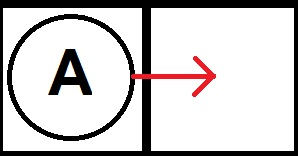
\includegraphics[scale=0.5]{PrzykladWykluczenie2}
        \centering
        \caption{Przykład wykluczania się akcji aktywnych z podtrzymującymi}
        \label{PrzykladWykluczenie2}
    \end{figure}

    Na pierwszy rzut oka wydawać by się mogło, iż niemożliwym jest wygenerowanie dwóch akcji znajdujących się w relacji wykluczania dla przykładu 
    \ref{PrzykladWykluczenie2}, jednakże istnieją dwie takie pary: 
    \begin{equation}
        zostan(na(A,lewy)),ruch(A,lewy,prawy)
    \end{equation} 
    oraz 
    \begin{equation}
        zostan(pusty(prawy)) oraz ruch(A,lewy,prawy)
    \end{equation} 
    Wynika to z faktu, iż zbiór efektów jednej akcji z powyższych par jest negowany przez drugi. Zbiorem efektów akcji 
    $zostan(na(A,lewy))$ jest $na(A,lewy)$, jednakże zbiorem efektów $ruch(A,lewy,prawy)$ jest ciut większy zbiór:
    \begin{equation}
        na(A,prawy), \sim na(A,lewy), pusty(lewy), \sim pusty(prawy)
    \end{equation}
    Widać, iż efekt $\sim na(A,lewy)$ jest negacją efektu $na(A,lewy)$. Akcje podtrzymujące i aktywne względem tego samego obiektu zawsze sobą ze sobą 
    w relacji wykluczającej ze względu na \textbf{niespójny efekt}.

    \begin{figure}[H]
        
\includegraphics[scale=0.5]{PrzykladWykluczenie1}
        \centering
        \caption{Przykład świata, w którym każdy z robotów próbuje przesunąć się na sąsiadujący z lewej strony klocek. Uwidoczniona sytuacja 
        jest przykładem wykluczających się akcji}
        \label{PrzykladWykluczenie1}
    \end{figure}

    Idea przedstawiona na rysunku \ref{PrzykladWykluczenie1} jest ciekawym przykładem, pozwalającym zrozumieć dokładniej definicję słowa 
    \textbf{równoległość} odnośnie planów generowanych przez GRAPHPLAN. Gdyby roboty poruszając się z tą samą szybkością ruszyły w tym samym momencie
    to wykonanie ów sekwencji akcji byłoby w zupełności możliwe, jednakże w sekcji \ref{Rownoleglosc} wspomniano, iż każdy z wygenerowanych planów 
    musi być możliwy do przedstawienia w postaci porządku liniowego, czyli plan równoległy może zostać przerobiony w dowolny sposób na plan,
    w którym każda z akcji wykonywana jest po kolei. Zgodnie z omawianym przykładem sprowadzenie ów planu do dowolnej postaci liniowej jest 
    niemożliwe, gdyż istnieje konfiguracja, w której to najpierw robot B miałby wykonać ruch, jednakże jest to niemożliwe ze względu na 
    obecność robota A na kafelku będącym jego celem podróży. Dodatkowe wprowadzenie ograniczeń na konwersję planów równoległych na liniowe 
    jest bardziej skompilowanym zagadnieniem, którego omówienie nastąpi w sekcji odpowiedzialnej za możliwe rozwinięcia algorytmu.
    
    Z powyższego opisu wynika, iż 
    omawiane relacje ruchu są ze sobą w relacji wzajmenie wykluczającej z powodu \textbf{przeszkadzania}. 
    Klocek A do wykonanaia ruchu potrzebuje znajdować się na kafelku środkowym, co oznacza, iż kafelek środowy musi byc niepusty, 
    jednakże klocek B potrzebuje, aby ów klocek był pusty. Relacja wykluczająca między tymi stanami bezpośrednio generuje wykluczanie się tych akcji.
    
    Ponadto, omawiane akcje w ilustracji \ref{PrzykladWykluczenie1} znajdują się w relacji wykluczającej z powodu \textbf{Konkurencyjnych potrzeb}. 
    Robot B przy przesunięciu \textbf{na} środkowy kafelek wymaga, aby on był pusty, natomiast robot A przy przesunięciu \textbf{z} środkowego klocka 
    musi się na nim znajdować, czyli kafelek musi być niepusty. Stany pusty i niepusty względem kafelka są w oczywistej relacji wykluczającej 
    co automatycznie generuje wykluczenie się wspomnianej pary akcji. Przykład ów przedstawia, iż jedna para akcji może być ze sobą w relacji wykluczającej 
    z kilku powodów, jednakże algorytm rozpatrując parę akcji podchodzi do tego w sposób binarny, co oznacza, iż patrzy jedynie czy znajdują się w 
    relacji wykluczającej czy nie, nie interesuje go liczba sposobów, na które ów relację można utworzyć.    

    Należy zauważyć, iż dzięki wprowadzeniu relacji wzajemnego wykluczania pozbyto się porównań wielu akcji, których zajście jest niemożliwe w tej samej 
    warstwie grafu. Koszt jaki został poniesiony ze względu na zapamiętywanie dodatkowych informacji o relacjach między akcjami jest często zaniedbywalny,
    ze względu na ogrom benefitów w postaci mniejszej liczbie sprawdzeń, a co za tym idzie- szybsze działanie algorytmu.


\section{Wyszukiwanie planu}
    Zdefiniowawszy wszystkie niezbędne elementy planera należy wskazać, w jaki sposób przy posiadaniu całej wiedzy wygenerowanej przez graf planujący.
    Wykonywane jest to w następujący sposób:
    \begin{enumerate}
        \item Rozpoczynając od stanu początkowego, zgodnie z opisanymi w poprzednich sekcjach metodami, odbywa się generowanie kolejnych warstw grafu,
        biorąc pod uwage informację o \textbf{mutexach} między akcjami oraz stanami
        \item Dla każdej nowo utworzonej warstwy $i$ dokonywane jest sprawdzenie, czy wszystkie założenia z celu nie znajdują się 
        w ów poziomie stanów. Jeśli odpowiedź jest negatywna, odbywa się dalsze generowanie planu zgodnie z 1. Jednak, gdy 
        wszystkie stany celu znajdują się na poziomie $i$ dochodzi do generowania planu.
        \item Dla każdego stanu z celów na poziomie $i$ dochodzi do wybrania akcji, dzięki której został on wygenerowany. 
        Ów operacja dokonywana jest dla każdego stanu. Jeżeli dobrane akcje są ze sobą w relacji wykluczającej, należy spróbować innej 
        kombinacji akcji. Jeśli wszystkie dobory akcji zawiodą należy wygenerować kolejną warstwę grafu i ponownie, w warstwie $i+1$, rozpocząc cały proces
        \item Jeśli jednak istnieje dobór akcji taki, że nie występuje między nimi relacja wykluczania, należy dla każdego stanu 
        znajdującego się w zbiorze warunków zajścia wspomnianych akcji wykonać procedurę z kroku 3. 
        \item Jeśli dojdzie do niepowodzenia na którymkolwiek z etapów powrotu do stanu wyjściowego algorytm podejmuje próbuję odpowiedniego dobrania 
        akcji na ostatnio sprawdzonym poziomie. Brak niepowodzenia na ścieżke powrotu od warstwy $i$ do warunków początkowych świadczy o tym, 
        iż istnieje sekwencja akcji pozwalająca otrzymać stany zdefiniowane z celu w określonym przez stany początkowe świecie, co oznacza, 
        iż jest możliwym utworzenie odpowiedniego \textbf{planu}.
    \end{enumerate}
    Aby precyzyjnie przedstawić działanie algorytmu w następnej części programu przeprowadzono rozbudową analizę konkretnego przykładu:

    \begin{figure}[H]
        
\includegraphics[scale=0.5]{PrzykladPlan1}
        \centering
        \caption{Sytuacja początkowa świata, dla którego odbędzie się przykładowe generowanie planu. Kolorem niebieskim zaznaczono kafelek docelowy robota}
        \label{PrzykladPlan1}
    \end{figure}

    \ref{PrzykladPlan1} przedstawia świat, w którym robot A z kafelka 1 próbuje przedostać się do kafelka 3 (Kafelki ponownie numerowane są od lewej strony
    do prawej).

    \begin{figure}[H]
        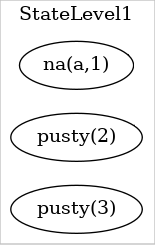
\includegraphics[scale=0.5]{PrzykladPlanStateLevel1}
        \centering
        \caption{Warunki początkowe omawianego świata. Obrazki ułatwiające analizę przykładu w całości zostały 
        wykonane przez oprogramowanie utworzone na rzecz pracy. }
        \label{PrzykladPlanWP}
    \end{figure}

    Ze względu na fakt, iż w języku programowania \textbf{PROLOG}, w którym implementowany jest algorytm, zmienne są oznaczane przy pomocy wielkiej litery,
    a stałe przy pomocy małej, wielkość litery w oznaczaniu nazwy robota nie ma istotnego znaczenia. Zwyczajowo w opisie robot będzie określany 
    przy pomocy wielkiej litery (np. \textbf{A}) natomiast w wygenerowanych przez program grafach przy pomocy małej \textbf{a}.
    W powyższy sposób zaprezentowano stan początkowy świata. Wszystkie definicje relacji takich jak \textbf{na}, \textbf{idz}, \textbf{zostan}, czy 
    \textbf{pusty} wprowadzono w podrozdziałach \ref{RozdzialWarunkiPoczatkowe} i \ref{RozdzialAkcje}. W wygenerowanych przez oprogramowanie grafach \textbf{poziomy stanów}
    określane są poprzez swój angielski odpowiednich \textbf{StateLevel}. Podobnie z \textbf{poziom akcji} i \textbf{ActionLevel}. 

    \begin{figure}[H]
        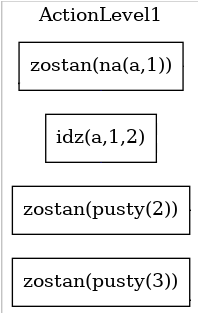
\includegraphics[scale=0.5]{PrzykladPlanActionLevel1}
        \centering
        \caption{Wygenerowane akcje na podstawie warunków początkowych}
        \label{PrzykladPlanAP1}
    \end{figure}

    Następnie przystąpiono do wygenerowania wszystkich możliwych akcji. Postąpiono zgodnie ze wskazówkami z podrozdziału \ref{RozdzialAkcje}. 
    Dodajemy niezbędne krawędzie wynikające z warunków, jak i efektów każdej z akcji oraz mutexy (oznaczone przerywanymi, niebieskimi liniami).

    \begin{figure}[H]
        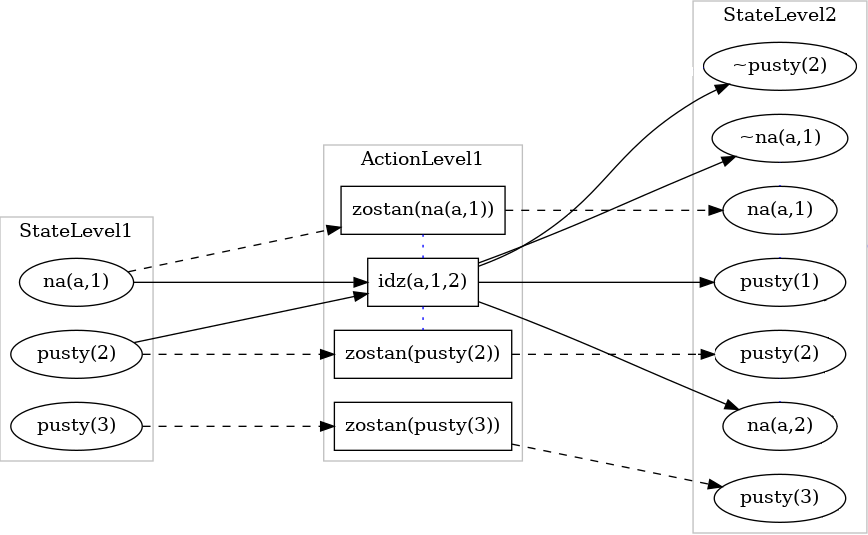
\includegraphics[scale=0.5]{PrzykladPlanWarstwa1}
        \centering
        \caption{Wygenerowany drugi stan grafu bezpośrednio wynikający z pierwszego poziomu akcji}
        \label{PrzykladPlanW1}
    \end{figure}

    Przy pomocy efektów akcji automatycznie wykreowano następny poziom stanów. Zgodnie z schematem planowania należy sprawdzić, czy oczekiwany cel
    $na(A,3)$ znajduje się w zbiorze stanów poziomu drugiego. Po szybkiej analizie okazuje się, iż cel nie znajduje się na wskazanym poziomie, więc
    należy dokonać rozszerzenia grafu planującego o kolejny poziom. Następuje to w sposób analogiczny.

    \begin{figure}[H]
        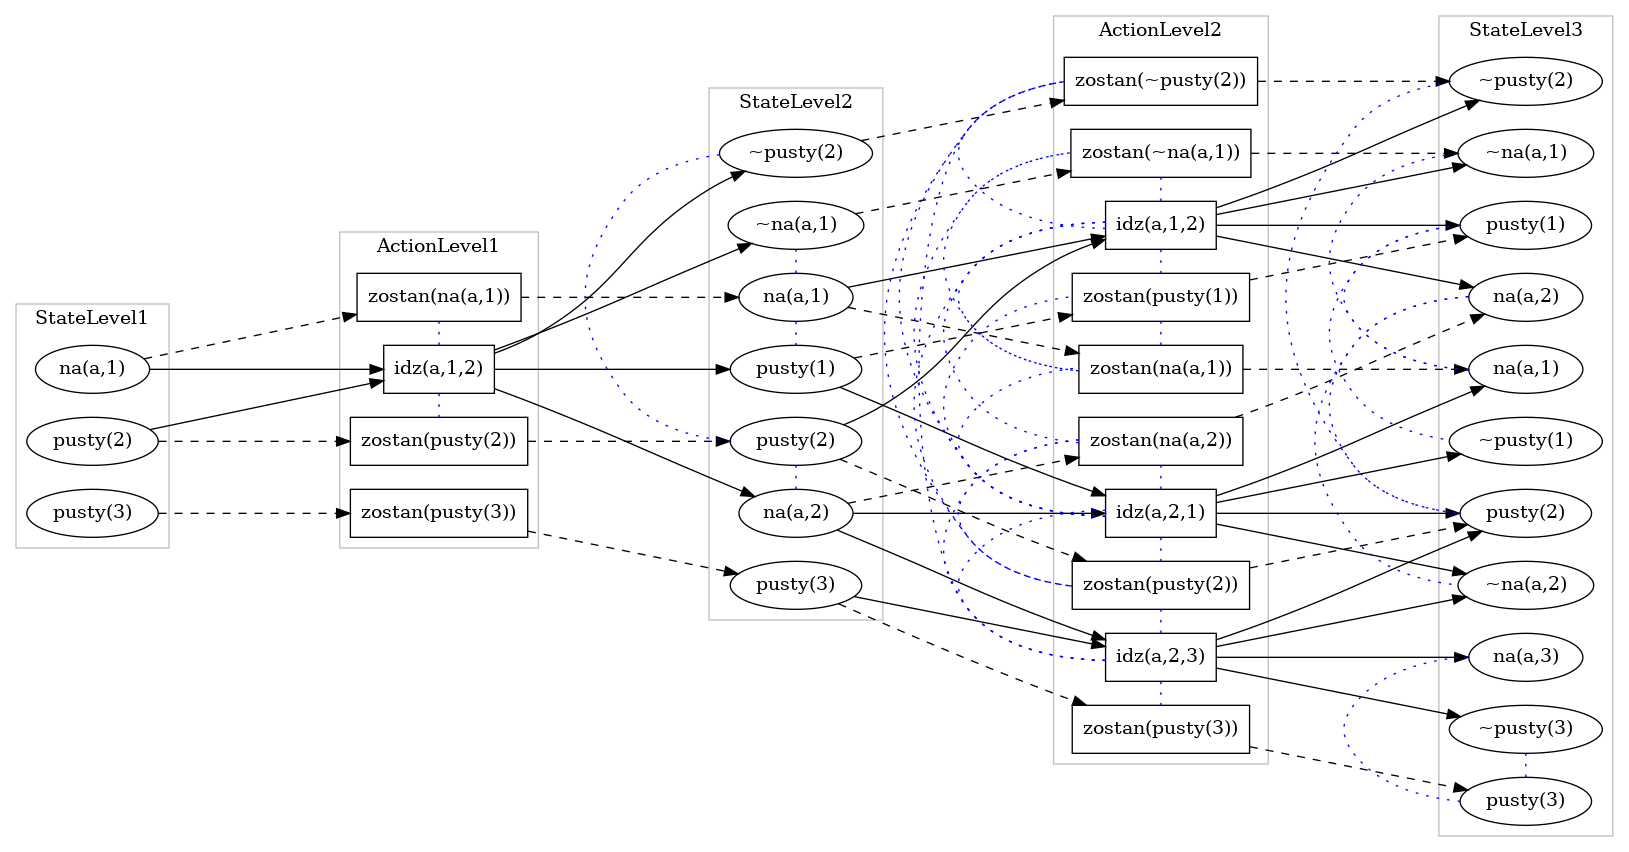
\includegraphics[scale=0.25]{FULL_GRAPHPLAN.DEMO1.gv}
        \centering
        \caption{Przykład kolejnej iteracji algorytmu}
        \label{PrzykladPlanW1}
    \end{figure}

    Po wygenerowaniu kolejnej warstwy algorytmu oraz zaznaczeniu wszystkich mutexów zauważono, iż stan $na(A,3)$ znajduje się w zbiorze stanów 
    \textbf{StateLevel3}. Następnym krokiem jest sprawdzenie, czy taki zbiór akcji, który doprowadzi nas do stanu $i-1$ bez wprowadzania żadnych sprzeczności.
    Okazuje się, iż istnieje taka para akcji: $idz(A,2,3) oraz zostan(pusty(1))$. Zgodnie z schematem generowania planu należy zejść iteracyjnie aż do 
    warunków początkowych aby uzyskać poprawny plan. W omawiany przykładzie łatwo zauważyć, iż przy pomocy akcji $idz(A,1,2)$ oraz $pusty(3)$ udało się 
    z powrotem otrzymać stan początkowy. Ze względu na fakt, iż człowiek jest w stanie sprawnie wydedukować akcje podtrzymujące na podstawie 
    akcji aktywny dla każdego poziomu, przy graficznym przedstawieniu planu (w formie opisowej i graficznej) z reguły akcje podtrzymujące będą 
    pomijane.

    \begin{figure}[H]
        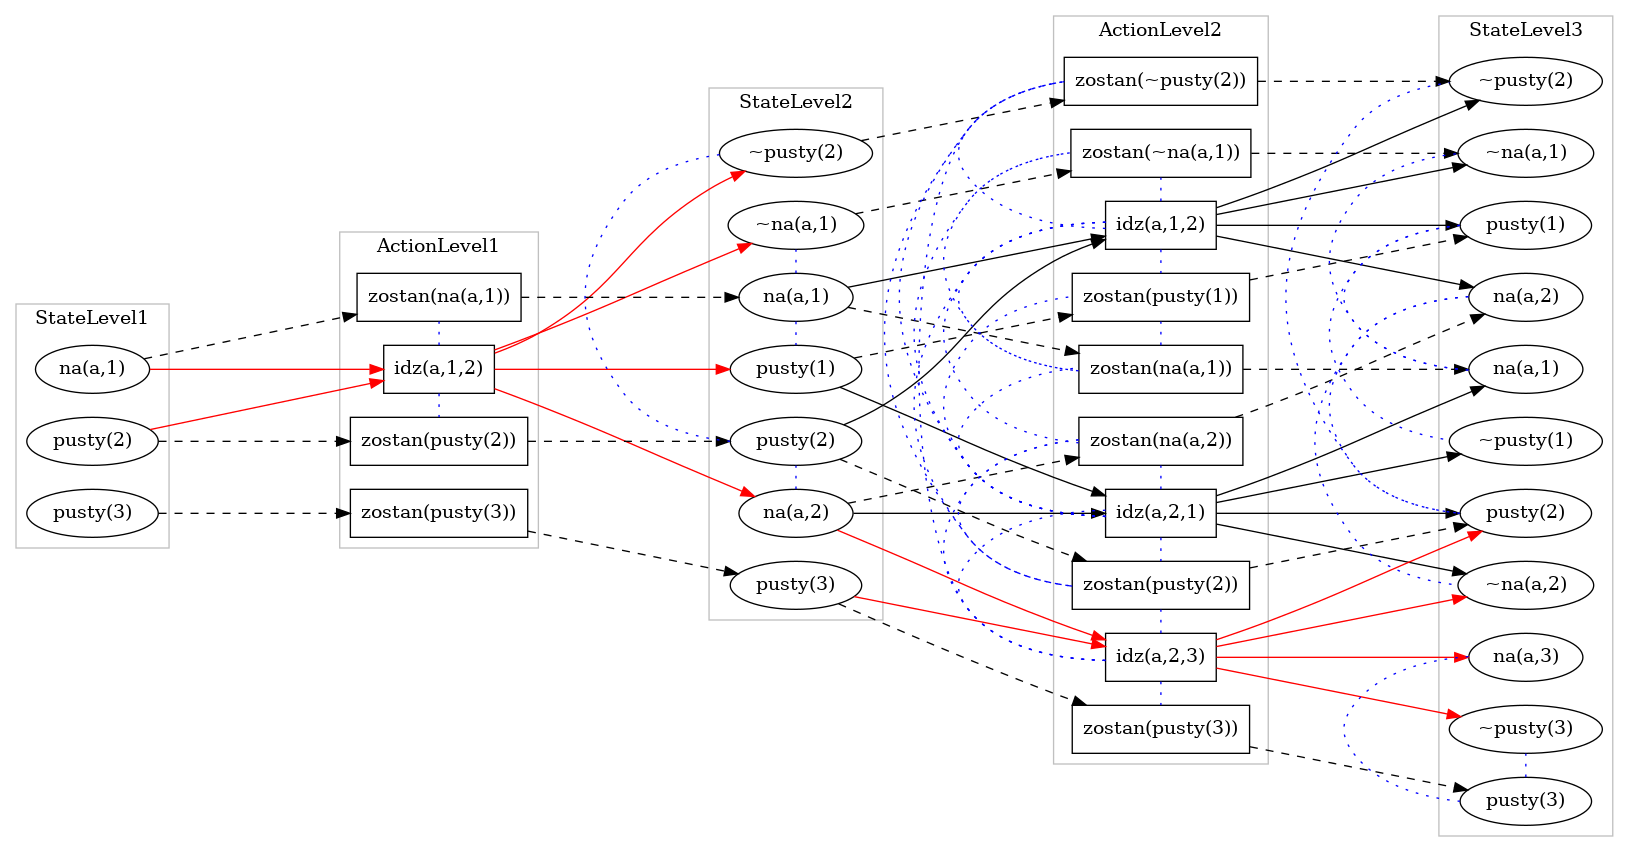
\includegraphics[scale=0.25]{FULL_GRAPHPLAN_DEMO2.gv}
        \centering
        \caption{Graf planujący z zaznaczonymi akcjami aktywnymi prowadzącymi do uzyskania wskazanego celu}
        \label{PrzykladPlanW1}
    \end{figure}

    Powyższy rysunek przy pomocy czerwonych strzałek przedstawia akcje aktywną, wraz z jej bezpośrednimi warunkami zajścia oraz efektami, które 
    prowadzą do uzyskania planu. Zgodnie z intuicją, najbardziej optymalny plan przeniesienia robota A z kafelka 1 na kafelek 3 to:
    \begin{equation}
        [[idz(A,1,2)],[idz(A,2,3)]]
    \end{equation}
    Ze względu na fakt, iż na danym poziomie może odbywać się więcej niż jedna akcja, każdy krok algorytmu oznaczany jest za pomocą \textbf{listy}, 
    którą możemy utożsamić z matematycznym zbiorem.

    W ten oto sposób wygenerowano poprawny plan stosując algorytm \textbf{GRAPHPLAN}.

\section{Własności GRAPHPLAN'u}
    Działanie GRAPHPLAN'u można przedstawić również jako swego rodzaju iteratywne przeszukiwane wszerz. 
    Dla każdego poziomu generowane są wszystkie możliwe stany, by następnie móc sprawdzić, czy cele do osiągnięcia 
    znajdują się w utworzonym zbiorze. Jeśli rzeczone cele nie znajdują się, algorytm wykonuje kolejną iterację, 
    poszerzając swoją wiedzę o świecie. Powyższe przeszukiwanie wykonuje się aż do momemntu, gdy uda się utworzyć satysfakcjonujący plan
    Dzięki tej własności łatwo pokazać, iż:
    \begin{theorem}
        Każdy wyprodukowany plan przez algorytm GRAPHPLAN jest planem legalnym, czyli spełnialnym dla zadanych 
        warunków początkowych, akcji oraz celów. Ponadto, jeśli dla opisanego świata istnieje plan GRAPHPLAN zawsze go znajdzie.
    \end{theorem}
    oraz
    \begin{theorem}
        Algorytm zawsze zwraca najkrótszy plan, czyli plan optymalny.
    \end{theorem}

    \begin{proof}
        W pierwszym kroku algorytm generuje nowy poziom stanów. Następnie sprawdza, czy cele znajdują się wśród stanów. Jeśli odpowiedź jest twierdząca,
        dobiera zbiór akcji, dzięki którym udało się spełnić postawione wymagania. Jeśli odpowiedź jest przecząca, algorytm generuje kolejną warstwę.
        Niech warstwa $i$ będzie warstwa, w której nie znajdują się wszystkie stany ze zbioru determinowanego przez zdefiniowane cele. W tym przpyadku
        dla $i+1$ warstwy algorytm próbuje wygenerować plan cofając się do stanu $i$. Jeśli uda się odpowiednio dobrać akcje 
        cofa się jeszcze dalej aż do stanu początkowego i kończy działanie, jako wynik zwracając plan. Powyższy opis determinuje optymalność planu.
    \end{proof}


    Ponadto należy się również przyjrzeć mechanizmom kreowania kolejnych stanów dla poszczególnych warstw. Algorytm robi to przyrostowo. 
    Wszystkie istniejące już stane przenoszone są przy pomocy akcji podtrzymujących do następnej warstwy, natomiast akcje aktywne produkują 
    nowe efekty- dodające bądź usuwające. Mimo iż akcja z perspektywy człowieka jest \textbf{usuwająca}, 
    z perspektywy komputera jest kolejną informacja, która również zostaje dodana do zbioru stanów.

    Korzystając z powyższej własności sformułowano następujący wniosek:
    \begin{theorem}
        \label{LevelOff}
        Liczba stanów w warstwie \textbf{i+1} jest zawsze większa bądź równa liczbie stanów w warstwie \textbf{i}
    \end{theorem}
    Skutki ów twierdzenia są dobrze uwidocznione w przykładach grafów planujących takich jak \ref{PrzykladPlanW1}.
    Twierdzenie \ref{LevelOff} generuje ciekawy wniosek. Niech oznaczenie $WSL(i)$ oznacza liczbę stanów wchodzą w skład $i$-tej warstwy.

    \begin{lemma}
        $\exists k\in\mathbb{N}$  $\forall i>k, i\in\mathbb{N}$ : WSL(i+1) = WSL(i)
    \end{lemma}

    Co sprowadza się do tego, iż od pewnego momentu liczba stanów dla każdej kolejnej warstwy jest stała.

    \begin{proof}
        Zgodnie z \ref{LevelOff} wiadomym jest, iż zawsze spełniona jest zależność $WSL(i+1) > WSL(i)$. Należy pokazać, iz od pewnego momentu 
        liczby stanów w warstwach dążą do stałej liczby. Ze względu na strukturę języka STRIPS istnieje skończona liczba akcji. W ów modelu nie istnieją
        akcje niedeterminstyczne, bądź jakiekolwiek niespodziewane efekty uboczne przeprowadzonych akcji. 
        Algorytm również rozpoczyna pracę z góry znaną liczbą obiektów, a każdy z obiektów może znajdować się w skończonej liczbie stanów takich 
        jak $na$ czy $pusty$. Algorytm rozszerza kolejne poziomy stanów przy pomocy akcji aktywnych, jednakże na podstawie skończonej 
        liczby obiektów oraz skończonych stanów, w jakich ów obiekty mogą się znajdować algorytm, dla każdego z obiektów, może wywnioskować jedynie skończoną 
        liczbę akcji, które może wykonać. Ostatecznie sprowadza się to do sytuacji, w której ze względu na skończoność wszystkich określonych dziedzin,
        $i$-ty poziom stanów algorytmu zawiera wszystkie możliwe stany dla wszystkich możliwych obiektów.
        Od tego momentu mimo przeprowadzania kolejnych akcji podtrzymujących bądź 
        aktywnych nie powstają już kolejne stany, gdyż zbiór efektów każdej z akcji ma już swoje odwzorowanie w poprzedniej warstwie. 
        Stąd wniosek, iż istnieje 
        moment krytyczny, dla którego dochodzi do stabilizacji liczby stanów w danej warstwie.
    \end{proof}

    \begin{definition}
        \textbf{Spłaszczeniem} algorytmu jest sytuacja, w której wygenerowanie kolejnego stanu nie prowadzi 
        do uzyskania nowych informacji o świecie.
    \end{definition}

    Powyższy lemat jest kluczowym w kontekście rozwiązywania tak zwanego \textit{Problemu stopu} dla algorytmu GRAPHPLAN.

    \subsection{Problem stopu}
    \begin{figure}[H]
        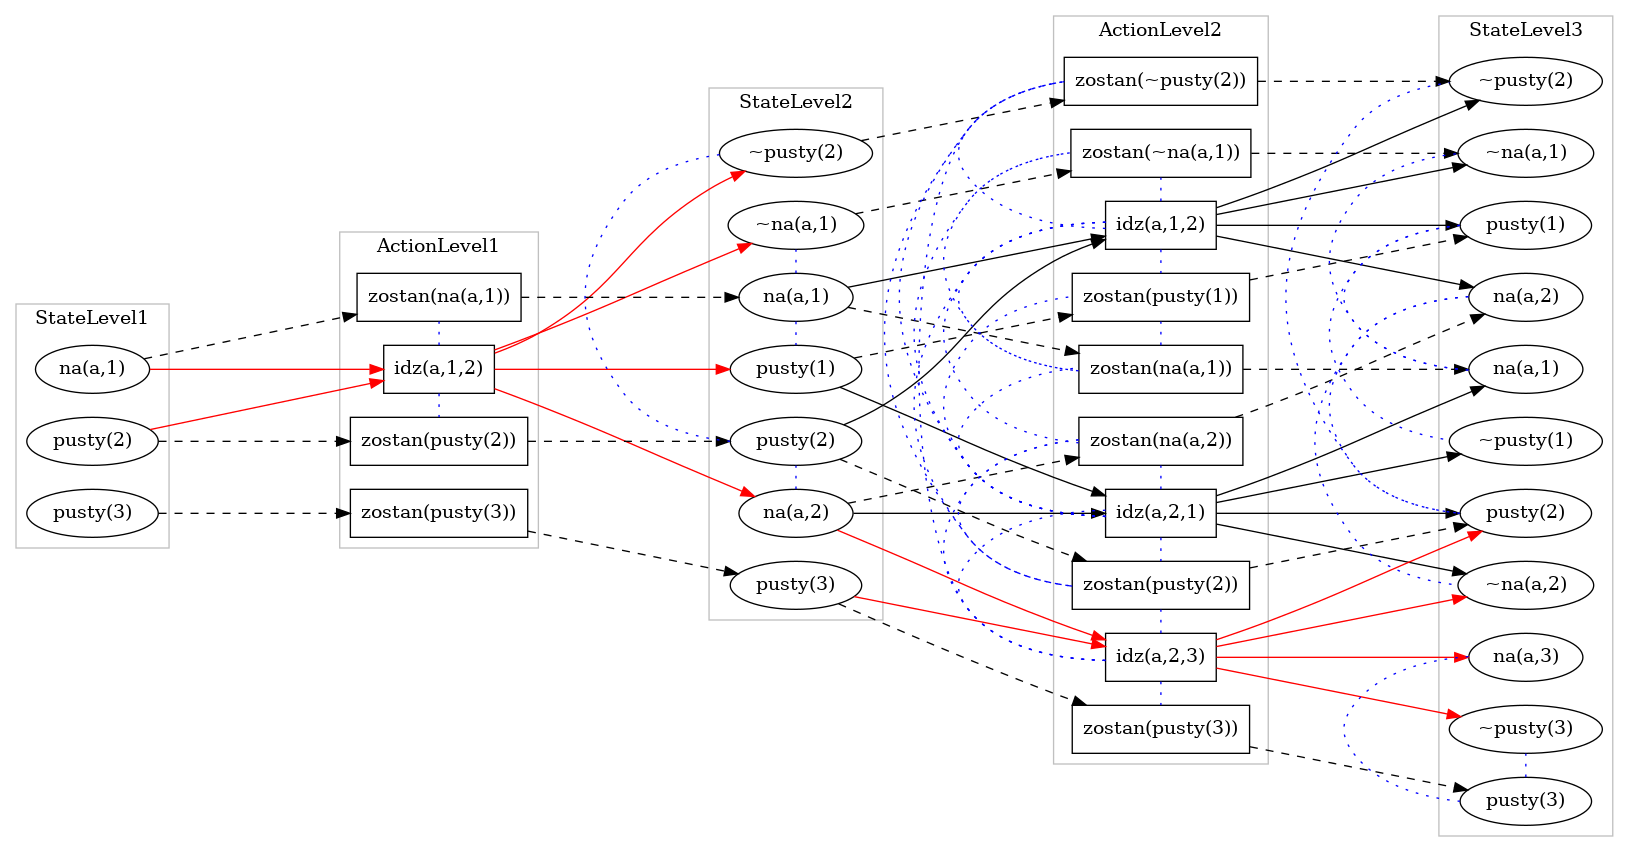
\includegraphics[scale=0.25]{FULL_GRAPHPLAN_DEMO2.gv}
        \centering
        \caption{Przykład świata, w którym osiągnięcie celu, którym jest kafelek oznaczony kolorem takim jak kolor użytej czcionki do oznaczenia 
        sygnatury robota, jest niemożliwe ze względu na absencję jednego z kafelków, będących łącznikiem, między robotem a jego celem.}
        \label{PrzykladPlanW1}
    \end{figure}
    Wcześniejsze przykłady rozpatrywały jedynie sytuację, w której algorytm zawsze znajdował plan, gdyż przedstawione światy były spreparowane w taki sposób, 
    aby rzeczony plan zawsze istniał. Jednakże nie zawsze musi tak być, więc należy zabezpieczyć algorytm również i przed taką ewentualnością. Łatwo zauważyć, 
    iż obecna struktura planu nie została utworzona z myslą o takiej sytuacji- algorytm będzie generował coraz to nowsze warstwy bezskutecznie próbując uzyskać 
    plan dla zdefiniowanego celu.Ostatecznie dojdzie do całkowitego zapętlenia pracy algorytmu. 
    Z tego powodu pierwszym pomysłem na uzbrojenie algorytm w mechanizm detekcji nieskończonej pętli jest sprawdzenie rozmiaru zbioru stanów dla dwóch 
    następujących po sobie warstw. Jeśli warstwa nowsza składa się z większej liczby stanów, algorytm uzyskuje nowe informacje o świecie i jest 
    przygotowany do dalszego trawersowania po grafie planującym, jednakże gdy ów liczby są sobie równe dochodzi do swego rodzaju stagnacji- wszystkie 
    możliwe ruchy nie wprowadzają nowych informacji o świecie. Jeśli dla poprzedniego stanu nie udało się utworzyć planu, algorytm wnioskuje, iż 
    również dla tego, jak i przyszłych, utworzenie stanu będzie niemożliwe, co powoduje zwrócenie przez program informacji o braku 
    możliwości utworzenia odpowiedniego planu i jego terminację.

    Po wprowadzeniu powyższej modyfikacji możliwym jest wyciągnąć następujący wniosek 

    \begin{lemma}
        GRAPHPLAN zawsze kończy swoje działanie.
    \end{lemma} 

    TO-DO: Może bardziej "matematyczne" dowody, a nastepnie obrazowe opisy wraz z rysunkami?
    Wprowadzenie informacji o liczbie akcji oraz mutexów, wprowadzenie twierdzenia o 
    wielomianowości czasu utworzenia algorytmu GRAPHPLAN (niestety eksponencjalny, ale 
    jednak wielomianowy))


    


	\cleardoublepage
	
	\chapter{Programowanie ograniczeń}
\thispagestyle{chapterBeginStyle}

\section{Wprowadzenie}
    Programowanie ograniczeń (inna nazwa: technologia więzów) jest narzędziem wykorzystywanym do rozwiązywania 
    problemów z dziedzin kombinatoryki, sztucznej inteligencji, czy planowania jak i harmonogramowania zadań.
    W skład tego podejścia do programowania często wyróżnia się dwa elementy: ograniczenia (zwane również
    stałymi) oraz problem rozwiązywania ograniczeń (ang. Constraint Satisfaction Problem, CSP)
    Poniżej dokonano formalnego zdefiniowania powyższych komponentów:
    \begin{definition}
        \label{ConstraintProblem}
        \textbf{Problem rozwiązywania ograniczeń, CSP} jest następującą trójką:
        \begin{equation}
            CSP = (V,D,C)
        \end{equation}
        gdzie:

        $V = \{x_{1},x_{2},...,x_{n}\}$ oznacza zbiór zmiennych wykorzystywanych do opisu problemu

        $D = \{d_{1},d_{2},...,d_{n}\}$ oznacza zbiór dziedzin wyżej wspominanych zmiennych. W ramach 
        rozważań zawartych w rzeczonej pracy rozpatrywane będą takie $d_{i}$, które są zbiorami zawierającymi 
        skończoną liczbę potencjalnych wartości zmiennej $x_{i}$.

        $C = \{c_{1},c_{2},...,c_{m}\}$ oznacza zbiór ograniczeń
    \end{definition}
    \begin{definition}
        \label{Constraint}
        \textbf{Ograniczenami} (inne nazwy: stałe, więzy) nazywamy zmienne oraz zależności między nimi, które muszą zostać spełnione 
        w ramach rozwiązywania problemu ograniczeń. Określamy je przy pomocy pary: 
        \begin{equation}
            C = (S,R)
        \end{equation}
        gdzie:

        S jest krotką wszystkich zmiennych wchodzących w skład relacji 

        R jest relacją, która definiuje jakie wartości mogą przyjąc zmienne, które w niej uczestniczą.
    \end{definition}
    Relacje często przedstawia się przy pomocy zbioru zawierającego krotki, które składają się ze wszystkich 
    przyporządkowań wartości do odpowiednich zmiennych.
    Przy następujących definicjach oczekiwanym celem będzie utworzenie mechanizmu rozwiązującego zadany problem. Jego wynikiem 
    będzie zbiór wszystkich zmiennych, oraz krotek, które będą zawierały odpowiednie wartości przyporządkowane dla zmiennych.
    \begin{definition}
        \label{Krotka}
        \textbf{Krotka} (ang. tuple) - struktura danych, która w systemach informatycznych odzwierciedla uporządkowany ciąg wartości
    \end{definition}
    Dodatkowo wprowadza się termin \textbf{arności} ograniczenia:
    \begin{definition}
        \label{Krotka}
        \textbf{Arność ograniczenia} (ang. arity)  związana jest z liczbą unikalnych zmiennych, która w nią wchodzi.
    \end{definition}
    Najpopularniejszymi typami ograniczeń są:
    \begin{enumerate}
        \item Ograniczenia o arności 1, zwane ograniczeniami \textbf{unarnymi} (w tym przypadku z reguły będą one ściśle związane z dziedziną, raczej 
        nie będą występowały w kontekście ograniczeń)
        \item Ograniczenia o arności 2, zwane ograniczeniami \textbf{binarnymi}
        \item Ograniczenia o arności 3, zwane ograniczeniami \textbf{ternarnymi}
    \end{enumerate} 

    Tak jak ograniczenie może mieć swoją arność, tak dla CSP również zdefiniowano pojęcie arności w lekko zmodyfikowany sposób 
    \begin{definition}
        \textbf{Arność} CSP o wartości $i$ zawiera w sobie wszystkie typy ograniczeń od arności 1 aż do arności $i$
    \end{definition}

    Wedle powyższego binarne CSP zawiera w sobie jedynie ograniczenia unarne jak i binarne.
    \begin{example}
        \label{CP1}
        Niech będzie dane równanie $x+y=z$, gdzie $x,y,z \in \{0,1\}$. Łatwo zauważyć, iż zadane równanie jest automatycznie ograniczeniem 
        wpływającym na prezentowane zmienne. Przyporządkowując odpowiednie wartości do zbiorów z definicji \label{ConstraintProblem} otrzymano
        \begin{enumerate}
            \item $ V = \{x,y,z\} $
            \item $ D = \{d_{x},d_{y},d_{z}\}$, gdzie $d_{x},d_{y},d_{z} = \{0,1\}$
            \item $ C = \{x+y=z\}$
        \end{enumerate}
        \textbf{Arność} ograniczenia występujące w przedstawionym przykładzie wynosi 3, determinowane jest to liczbą zmiennych, która wchodzi w jej skład.
        Rozwiązaniem tego problemu będą następujące dopasowania:

        
        $((x,y,z),\{0,0,0\}, \{1,0,1\}, \{0,1,1\})$

    \end{example}
    Odnalezienie rozwiązań z przykładu \ref{CP1} było trywialne ze względu na małą liczbę zmiennych, wąskie dziedziny oraz tylko jedno wprowadzone ograniczenie.
    Podobnie jak z planowaniem, wprowadzenie dodatkowych zmiennych, powiększanie dziedzin oraz zbioru ograniczeń znacznie wpływa na skomplikowanie 
    odnajdowania rozwiązania.



\section{Pojęcie ustalenia i spójności}
    \label{SpójnośćRodział}
    W ostatecznej formie problem ograniczeń wyszukuje rozwiązanie przy pomocy ustalenia wartości zmiennych, jednakże naistotniejsza 
    jest droga, jaką pokonuje, aby ów ustalenia uzyskać. W tej sekcji należy wprowadzić kilka dodatkowych definicji:
    \begin{definition}
        Ustalenie zmiennych jest \textbf{spójne}, gdy nie jest w konflikcie z żadnym z ograniczeń.
    \end{definition}
    Ustalenie spójne również w nomenlakturze programowania ograniczeń nazywane jest ustaleniem \textbf{legalnym}.
    Nadanie zmiennym X oraz Y wartość 1 w przykładzie \ref{CP1} prowadzi do konfliktu, gdyż nie istnieje wartość 2 w zbiorze $D_{z}$.
    \begin{definition}
        \textbf{Kompletnym ustaleniem} nazywamy takie ustalenie, w którym wszystkie zmienne posiadają ustaloną wartość.
    \end{definition}
    Łatwo zauważyć, iż kompletne ustawienie jest jednocześnie rozwiązaniem problemu ograniczeń. Z tego płynie następujący wniosek:
    \begin{corollary}
        Każde rozwiązanie problemu ograniczeń jest spójne.
    \end{corollary}

    Dodatkowo w źródłach \cite{AI} definiuje się częściowe ustalenie oraz częściowe rozwiązanie. Zgodnie z nazewnictwem 
    częściowe ustalenie związane jest z sytuacją, gdy jeszcze nie wszystkie zmienne mają dokładnie określone wartości, natomiast 
    częściowe rozwiązanie w praktyce identyfikuje się jako spójne częściowe ustalenie.

    Po wprowadzeniu powyższych definicji należy rozpocząć rozważania na temat tego, w jaki sposób 
    problem ograniczeń może zostać rozwiązany. Pierwszym z podejść może być ustalenie wartości dla zmiennych poprzez 
    analizę ograniczeń, jakie między nimi występują. Ten proces nazywany jest \textbf{propagacją ograniczenia}. Dzięki 
    podstawowej analizie ograniczeń algorytm może wyeliminować wartości nadmiarowe znajdujące się w zadanych dziedzinach, co znacząco wpłynie 
    na przyszłościowe osiągi pod kątem czasowym. Często propagacja ograniczeń jest wykonywana jako \textit{preprocessing step}, czyli 
    jako krok, który zostanie wykonany jeszcze przed rozpoczęciem prawdziwej pracy nad problem. 
    
    Przy rozwiązywaniu problemów związanych z ograniczeniami bardzo intuicyjną reprezentacją, jest reprezentacja 
    w formie \textit{grafu}. Poprzez wierzchołki oznacza się zmienne wchodzące w skład problemu, natomiast poprzez krawędzie- 
    binarne ograniczenia, która między nimi występują. Z tego powodu pożądanym zabiegiem będzie przedstawienie wszystkich ograniczeń 
    n-arnych w formie binarnej.

    Kluczem do uzyskania poprawnego efektu propagacji ograniczeń jest skorzystanie z pojęcia zdefiniowanego jako \textbf{lokalna spójność}.
    Istnieją różne typy lokalnej spójności:
    \begin{itemize}
        \item \textbf{Spójność wierzchołkowa} (ang. node consistency) - Zmienna jest wierzchołkowo spójna, 
        gdy wszystkie wartości znajdujące się w jej dziedzine spełniają zdefiniowane przez nią ograniczenie unarne.
        Graf jest wierzchołkowo spójny, gdy wszystkie wierzchołki wchodzące w skład grafu są wierzchołkowo spójne.
        Zachowanie wierzchołkowej spójności z reguły sprowadza się do \textbf{zawężania} dziedziny zmiennej.
        \item \textbf{Spójność krawędziowa} (ang. arc consistency/edge consistency)- Zmienna jest spójna krawędziowo wtedy, 
        gdy każda wartość z jej dziedziny spełnia binarne ograniczenia zmiennej. Graf jest krawędziowo spójny gdy każda para 
        zmiennych jest ze sobą krawędziowo spójna.
        \item \textbf{Spójność ścieżki} (ang. path consistency) - Dwie zmienne $a,b$ są spójne w kontekście ścieżki z trzecią zmienną 
        $c$, gdy każde przypisanie wartości do zmiennych $a,b$ spełniające ograniczenie występujące między rzeczonymi zmiennymi dodatkowo 
        spełnia ograniczenie między zmiennymi $a,c$ oraz $c,b$.
        \item \textbf{K-spójność}- CSP jest k-spójne, gdy dla każdego spójnego ustalenia zawierającego $k-1$ zmiennych można dołączyć k-tą zmienną 
        bez załamiania spóności. Pojęcie 2-spójność jest tożsame z spójnością krawędziową, a 3-spójność- ze spójnością ścieżki.
    \end{itemize}

    Sprowadzanie problemu ograniczeń do sytuacji, w której zachodzi lokalna spójność jest określane mianem \textbf{propagacją ograniczeń}. 
    Jest to o tyle istotne, iż jedną z głównych metod rozwiązywania problemu ograniczeń jest sprowadzenie dziedzin zmiennych do pojedynczej wartości- 
    wtedy całkowitym ustaleniem jest nadanie zmiennej jedynej wartości w swojej dziedzinie. Propagacja ograniczeń jest silnym mechanizmem wykrywającym 
    niespójności- jeśli przy próbie propagacji któraś z wartości zostałaby z pustą dziedziną, wtedy należałoby przerwać rozwiązywanie problemu wraz 
    ze zwróceniem informacji o fakcie, iż nie ma takiego ustalenia zmiennych przy obecnych dziedzinach, dla którego rozpatrywane ograniczenie 
    jest rozwiązywalne.

\section{Ograniczenia globalne}
    W teorii programowania ograniczeń istnieją również ograniczenia zwane \textbf{globalnymi}. Mimo swojej nazwy, 
    globalne ograniczenia nie zawsze są związane ze wszystkimi zmiennymi wchodzącymi w skład problemu ograniczeń. 
    Ich istnienie warunkowane jest występowaniem w świecie rzeczywistym zależności, które często się powtarzają i nie są 
    unikalne dla jednego problemu. Przykładem takiego ograniczenia jest sytuacja, w której każda ze zmiennych ma mieć inną wartość.
    Formalniej mówiąc, wszystkie zmienne muszą być parami różne. Ów ograniczenie jest na tyle popularne, iż nosi ono swoją nazwę 
    \textbf{Alldiff} i jest często ograniczeniem wbudowanym w moduły zajmujące się programowaniem ograniczeń, co ułatwia i przyśpiesza 
    pracę użytkownika. Innym ograniczeniem z rodziny ograniczeń globalnych jest \textbf{ograniczenie zasobów}. Jak sama nazwa wskazuje, 
    rzeczone ograniczenie globalne wykorzystywane jest w modelowaniu sytuacji z dziedzin planowania bądź harmonogramowania zadań. 
    Przy rozwiązywaniu tego typu ograniczenia częstą metodą jest sumowanie wartości zmiennych wchodzących w skład dziedziny \cite{AI}.
    
    
\section{Wyszukiwanie rozwiązań}
    Podstawowa metoda rozwiązywania problem z dziedziny ograniczeń nosi miano metody \textbf{cofającej} (ang. backtracking).
    Działa ona zbliżenie do mechanizmu przeszukiwania grafu wgłąb. Na początku wybierana jest jedna ze zmiennych. Dla każdej wartości 
    z dziedziny dochodzi do częściowego ustalenia- zmienna otrzymuje wartość równą pierwszej wartości w swojej dziedzinie. Następnie, 
    korzystając z tej informacji dochodzi do propagacji ograniczeń. Jeśli wybrana została poprawna wartość propagacja ograniczeń doprowadzi 
    do znalezienia rozwiązania problemu. Istnieje również sytuacja, w której wybrana wartość prowadzi do slepego zaułka, czyli do sytuacji, w której 
    nie istnieje odpowiednie ustalenie zmiennych. Wtedy należy \textbf{cofnąć} 
    się do miejsca, w którym zmiennej nadaliśmy wartość i spróbować innego ustalenia. 
    Połączenie mechanizmu cofnięcia wraz z propagacją ograniczeń, czyli z utrzymywaniem lokalnej spójności na każdym etapie 
    wyszukiwania rozwiązania jest znakomitą techniką poprawiającą wydajność. Dzięki propagacji ograniczeń często 
    dochodzi do sytuacji, w której wyżej wymienione ślepe zaułki są eliminowane zanim mechanizm cofania je rozpatrzy. 
    
    Drugą metodą jest metoda nazywana \textbf{wyszukiwaniem lokalnym} (ang. local search). Metoda cofająca, jak sama nazwa wskazuje, próbowała dokonać 
    częściowego ustalenia, by następnie przy propagacji ograniczeń udowodnić, iż rozpatrywane częściowe ustalenie jest prawidłowe 
    i generuje odpowiednie całkowite ustalenie. Metodologia wyszukiwania lokalnego różni się w swojej filozofii tym, iż na samym 
    początku dochodzi do pełnego ustalenia zmiennych. W znacznej większości przypadków ów pełne ustalenie jest 
    nieprawidłowe, to znaczy nie spełnia wszystkich ograniczeń. Wtedy mechanizm próbuje na bieżąco naprawiać sytuację modyfikując całkowite ustalenie w takich 
    sposób, aby ustalenie nadal było całkowite jednocześnie spełniając ograniczenie, które wcześniej powodowało konflikty. Jeśli algorytm będzie w stanie 
    rozwiązać wszystkie ograniczenia uzyska odpowiednie ustalenie zmiennych.

    Porównując powyższe dwie metody łatwo zauważyć, iż różnią się one od siebie w znacznym stopniu, nie tylko w samej filozofii działania, lecz także 
    w efektach.

    \begin{definition}
        \label{AlgorytmKompletny}
        \textbf{Algorytmem kompletnym} jest algorytm, który gwarantuje uzyskanie rozwiązania oraz jest w stanie 
        wykryć, gdy takowe rozwiązanie nie istnieje
    \end{definition}

    Przeciwieństwem algorytmu kompletnego jest algorytm \textbf{niekompletny}, czyli taki, który nie gwarantuje 
    uzyskania optymalnego rozwiązania oraz wykrycia, czy problem posiada rozwiązanie. Algorytmy niekompletne natomiast są o wiele 
    szybsze oraz dobrze przybliżają optymalne rozwiązanie. 

    Zgodnie z powyższym metoda cofająca jest przykładem algorytmu kompletnego- systematycznie generuje nowe ustalenia oraz propagacje ograniczeń,
    natomiast wyszukiwanie lokalne jest przykładem algorytmu niekompletnego- łatwo sobie wyobrazić sytuację, iż naprawienie jednego ograniczenia 
    może nieustannie generować zepsucie kolejnego. W trakcie wyboru algorytmu ważnym jest, aby znać jego zalety jak i wady. Do implementacji 
    GRAPHPLANU został wykorzystany mechanizm cofania, aby zwracany przez algorytm plan był zawsze optymalny.



    Powyżej wymienione metody posiadają wiele dodatkowych usprawnień oraz specjalnie zdefiniowanych heurystyk,
    z którymi czytelnik może zapoznać się kierująć się do następującej pozycji w bibliografii \cite{CP}
    
\section{Programowanie w logice z ograniczeniami}
    Ze względu na wiele podobieństw w mechanizmach, jak i w samej idei, między technologią więzów a programowanie w logice, takich jak chociażby mechanizm cofania, który jest 
    powszechnie wykorzystywany w obu podejściach, zdecydowano się na utworzenie połączenia między nimi w celu uzyskania korzystniejszych wyników. Z tej kombinacji powstał 
    typ programowania nazywany \textbf{Programowaniem w logice z ograniczeniami}.
    \begin{definition}
        \textbf{Programowanie w logice z ograniczeniami} (ang. Constraint logic programming) jest jedną z form programowania ograniczeń,
        w której podstawowe mechanizmy programowania w logice zostały rozszerzone o koncpecje pochodzące z programowania ograniczeń.
    \end{definition}

    \begin{example}
        Programowanie ograniczeń zastosowane w języku PROLOG, który jest językiem programowania logicznego:
        
        \begin{lstlisting}[language=PROLOG, caption=Funkcja wypisująca liczby gdy ich suma jest większa od 0]
            FUNC(X,Y) :-
            X+Y > 0,
            writeln(X),
            wirteln(Y).
        \end{lstlisting}
    \end{example}
    W powyższym przykładzie zastosowano najprostsze z możliwych ograniczeń: wartość sumy zmiennych musi być większa od 0. 
    Ze względu na częste parowanie programowania ograniczeń z programowaniem w logice, wiele implementacji języków programowania w 
    logice implementuje gotowe moduły, które dostarczają technologię więzów dla różnych typów dziedzin. Dla przykładu, dla 
    jednej z najpopularniejszych implementacji języka programowania PROLOG dostępne są następujące moduły:
    \begin{itemize}
        \item clpfd- moduł, w którym dziedziny są skończone i składają się z liczb całkowitych. Ów moduł 
        wykorzystywany jest w zaimplementowanym algorytmie GRAPHPLAN
        \item clpb - moduł, w którym dziedziny składają się z wartości boolowskich
        \item clpq - moduł, w którym dziedziny składają się z liczb wymiernych w formie dziesiętnej
        \item clpr - moduł, w którym dziedziny składają się z liczb rzeczywistych zmiennopozycyjnych 
    \end{itemize}
    Dzięki powyższym modułom można tworzyć bardziej zmyślne ograniczenia niż zwykłe relacje równości, mniejszości bądź nierówności. Z przykładami takich zastosowań
    czytelnik będzie mógł się zapoznać w sekcji opisującej implementację algorytmu.

\section{Obrazowe przykłady}
    Przykładem realizacji problemu ograniczeń poprzez wykonanie operacji propagacji ograniczeń wraz z mechanizmem cofania będzie popularny \textbf{Problem plecakowy}
    \begin{example}
        \textbf{Dyskretny problem plecakowy}- (ang. discrete knapsack problem) problem wyboru przedmiotów w taki sposób, aby spełniały następujące założenia:
        \begin{itemize}
            \item suma wartości wybranych przedmiotów musi być jak największa 
            \item suma wag wybranych przedmiotów nie może przekraczać wartości plecaka
        \end{itemize}

    \end{example}

\section{Wykorzystanie w algorytmie}

    Podczas graficznego prezentowania przykładów programowania ograniczeń często wykorzystywaną strukturą był graf, chociażby w sekcji omawiającej 
    pojęcie lokalnych spójności (\ref{SpójnośćRodział}). Ze względu na ów powiązanie między programowaniem ograniczeń a GRAPHPLAN'em do podstawowego opisu GRAPHPLANU z rodziału 2 
    \ref{GRAPHPLANRozdzial} dodano funkcjonalności opisane w powyższych rozdziałach. 

    Każdy ze stanów oraz akcji zawiera w sobie dodatkowy \textbf{indykator}. Jest to liczba ze zbioru liczb całkowitych, o której 
    należy mysleć bardziej w kontekście wartości bool'owskich $\{prawda,fałsz\}$. Wartość liczby równa 0 indukuje fałszywość stanu, natomiast wartość większa od 0 indukuje jego
    prawdziwość. Przy pomocy indykatorów program ustala, które stany, bądź akcje 
    są w danej warstwie prawdziwe, czyli występują w świecie oraz takie, które w ów świecie w danym momencie nie występują, czyli są fałszywe. 
    Odbywa się to w następujący sposób:
    \begin{enumerate}
        \item Wszystkie stany wchodzące w stan początkowy otrzymują indykator równy 1, gdyż są aktualnie prawdziwe 
        w rozpatrywanym świecie.
        \item W trakcie generowania akcji następuje utworzenie powiązania między warunkami zajścia, akcjami oraz ich efektami.
        Akcja zostaje powiązane ze swoim warunkiem następującym ograniczeniem: wartośc indykatora akcji jest mniejsza bądź równa wartości 
        indykatora warunku. Należy to rozumieć w następujący sposób- jeśli warunek jest prawdziwy to akcja \textbf{może} zachodzić w świecie, natomiast 
        jeśli warunek jest nieprawdziwy, czyli ma indykator równy 0, akcja automatycznie dostaje indykator równy 0.
        Efekt zostaje powiązany ze swoją akcją poprzez następujące ograniczenie: jeśli jakakolwiek akcja w danej warstwie, 
        która ma dany stan za efekt zachodzi, wtedy również i efekt w nim występuje. Jeśli wszystkie akcje generujące ów efekt mają indykator równy 0 
        wtedy efekt nie może zachodzić na danym poziomie, więc również otrzymuje indykator równy 0.
        \item Dochodzi do sprawdzenia relacji wzajemnego wykluczania poprzez sprawdzenie indykatorów dwóch stanów- Jeśli ich iloczyn jest równy 0, wtedy 
        dwa stany nie mogą razem występować na danym poziomie.
        \item Przy dokładnej realizacji kroków 2 i 3 algorytm jest w stanie wygenerować kolejny poziom stanów. Po wygenerowaniu 
        dochodzi do sprawdzenia, czy wszystkie stany zawarte w zbiorze przechowującym cele mają indykatory równe 1. Jeśli nie, 
        rzeczony proces jest powtarzany aż do otrzymania pożądanego skutku.
        \item Gdy wszystkie cele otrzymają indykator 1, program przelicza wszystkie indykatory, dzięki czemu jest w stanie bezbłędnie określić, który 
        stan bądź która akcja na danym etapie przetwarzania świata znajdują się w nim bądź nie. Ów mechanizm jest silnie wykorzystywany 
        przy generowaniu grafów, przedstawiających zachodzące w świecie zmiany.
    \end{enumerate}

    Dzięki tej z pozoru niewielkiej modyfikacji algorytmu GRAPHPLAN zyskuje on zdecydowane przyśpieszenie w fazie kreowania planu. Gdy GRAPHPLAN dojdzie do odpowiedniego
    poziomu stanów, gdzie znajdują się wszystkie stany ze zbioru celów, wszystkie komponenty wchodzące w skład grafu planującego będą miały dodatkową informację o swojej prawdziwości 
    w danej warstwie. Odnalezienie planu sprowadza się do rozwiązania problemu ograniczeń dla wszystkich stanów grafu. Dokonywane jest to wedle myśli przewodniej GRAPHPLANU, czyli 
    poprzez mechanizm cofania wraz z propagacją ograniczenia przy zachowaniu lokalnej spójności. Bez tej modyfikacja wyłuskanie planu z grafu planującego przypominałoby wyszukiwanie 
    w głąb w grafie. Przechowywanie dodatkowej informacji w formie indykatora znacznie usprawnia ten proces.

    Dokładne sformuowanie ograniczeń przy pomocy symboli matematycznych odbędzie się w sekcji poświęconej implementacji algorytmu.
    


	\cleardoublepage
	
	\chapter{Implementacja}
\thispagestyle{chapterBeginStyle}

\section{Połączenia między komponentami}

\section{Implementacja algorytmu}

\section{Generowanie grafów}

\section{Interfejs użytkownika}

	\cleardoublepage
	
	\chapter{Instalacja i wdrożenie}
\thispagestyle{chapterBeginStyle}

\textbf{UWAGA:} Poniższy opis przedstawia sposób instalacji odpowiednich pakietów dla komputerów korzystających z systemu operacyjnego 
\textbf{Linux}, a dokładniej- dystrybucji \textbf{Ubuntu}. Użytkownik chcąc zainstalować aplikację wraz z jej komponentami na 
komputerze z innym systemem operacjnym zobowiązany jest do samodzielnego zapoznania się ze wszystkimi komendami bądź mechanizami 
umożliwającymi instalację wskazanych pakietów.

\section{Instalacja pakietu SWI-Prolog}
\label{SWI-PROLOGRozdzial}
    Korzystając z dystrybucji Linuxa o nazwie Ubuntu, wystarczającą czynnością do poprawnej instalacji pakietu SWI-Prolog jest uruchomienie 
    następującej komendy z poziomu linii komend \texttt{sudo apt install swi-prolog-core}.
    
    Należy pamiętać o wymogu posiadania praw adminsitratora na komputerze, na którym dokonywany jest proces instalacji.
    W momencie, w którym komputer zakończy pobieranie oraz instalację pakietu wprowadzenie komendy \textit{swipl} powinno spodoować uruchomienie 
    interaktywnego interpretera języka PROLOG. Jeśli powyższa czynność zakończyła się sukcesem, komputer jest gotowy do uruchomienia kodu źródłowego 
    algorytmu oraz rozpoczęcia pracy nad kreowanie odpowiednich planów
\section{Instalacja języka Python}
    \label{InstallPython}
    Większość dystrybucji Linuxa posiada wbudowany w sobie język programowania python. Z reguły można to zweryfikować poprzez wpisanie komendy 
    \texttt{python3 --version}
    Należy zauważyć, iż wszystkie komponenty zostały napisane dla wersji języka python 3.x. Użytkownik korzystając ze starszych wersji 
    może spotkać się z anomaliami negatywnie wpływającymi na funkcjonowanie aplikacji, dlatego zaleca się korzystanie ze wskazanej powyżej wersji. \\
    Do poprawnego uruchomienia aplikacji wymagane są następujaće biblioteki 
    \begin{itemize}
        \item Tkinter
        \item graphviz 
        \item PIL
        \item pyswip
    \end{itemize}
    Poniżej znajdują się odpowiednie komendy, których użycie z poziomu linii komend zagwarantuje poprawne uruchomienie aplikacji:
    \begin{listing}[H]
        \begin{verbatim}
            sudo apt install python3-tk
            pip3 install graphviz
            pip3 install Pillow
            pip3 install pyswip
        \end{verbatim}
        \caption{Instalacja odpowiednich bibliotek dla języka python}
    \end{listing}
    Przed uruchomienie powyższych komend użytkownik winien posiadać zainstalowany pakiet \textit{pip}. Jeśli pobieranie wskazanych bibliotek zakończy 
    się błędem, należy uprzednio wykonać następującą komendę: \texttt{sudo apt install python3-pip} .
    Całą aplikację również jest uruchamiana z poziomu linii komend. Po pobraniu odpowiednich plików, w folderze \texttt{sources} znajduje się plik
    \texttt{gui.py}, który zawiera kod rozruchowy interfejsu użytkownika. \\
    Będąc we wskazanym katalogu należy uruchomić terminal i wprowadzić następującą
    komendę: \texttt{python3 gui.py}
    Jeśli operacja zakończy się sukcesem, użytkownik powinien ujrzeć okienko identyczne do tego, które zostało przedstawione w ramach sekcji \ref{GUIRozdzial}

\section{Dokumentacja}
    W katalogu \texttt{sources} (patrz Dodatek~\ref{plytaCD}) znajduje się katalog \texttt{html}. W nim, przy pomocy popularnego narzędzia \textbf{Doxygen},
    który jest automatycznym generatorem dokumentacji dla wielu popularnych języków programowania (w tym także dla pythona), wygenerowano plik \\
    o nazwie 
    \texttt{index.html}. Naciśnięcie na ów plik dwukrotnie przy pomocy lewego przycisku myszy powinno uruchomić przeglądarkę, w której, w formie strony
    internetowej, zostanie użytkownikowi przedstawiona pełna dokumentacja zaimplementowanych mechanizmów. \\

    \begin{figure}[H]
        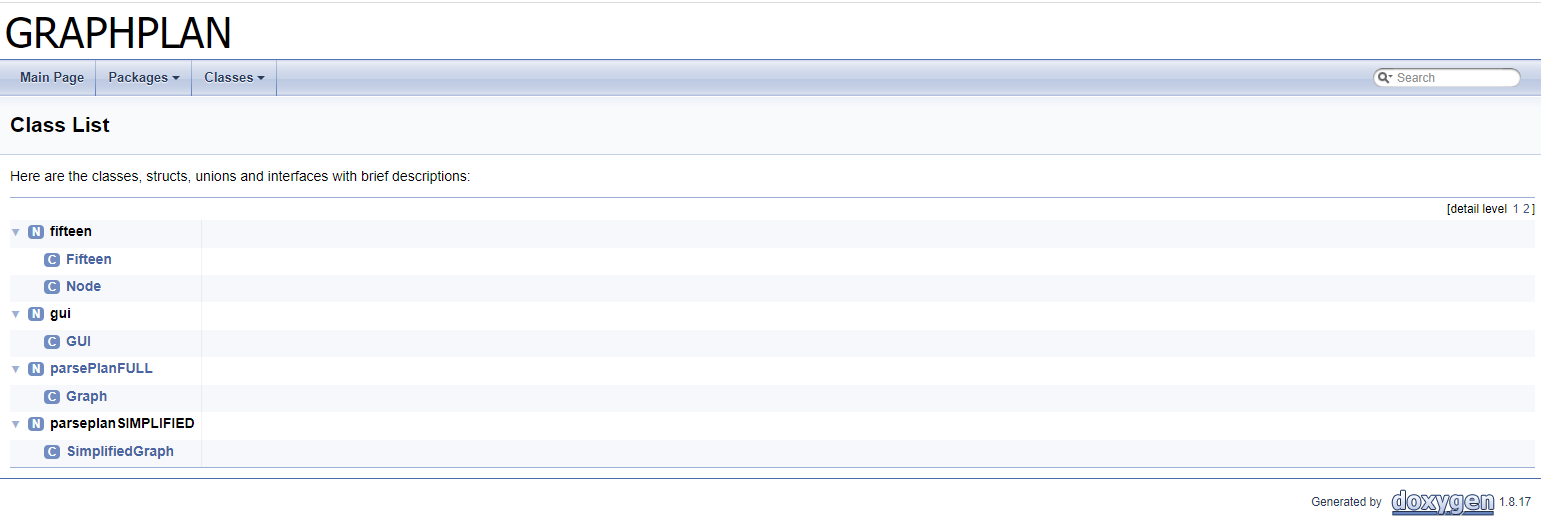
\includegraphics[scale=0.4]{SpisKlas}
        \centering
        \caption{Spis udostępnionych klas}
    \end{figure}

    \begin{figure}[H]
        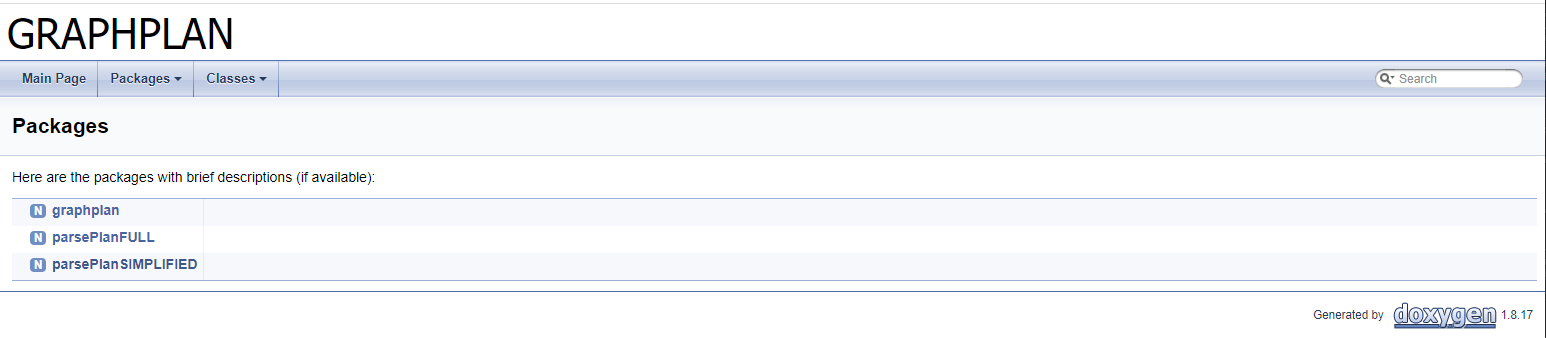
\includegraphics[scale=0.4]{SpisPaczek}
        \centering
        \caption{Spis udostępnionych paczek}
    \end{figure}

    \begin{figure}[H]
        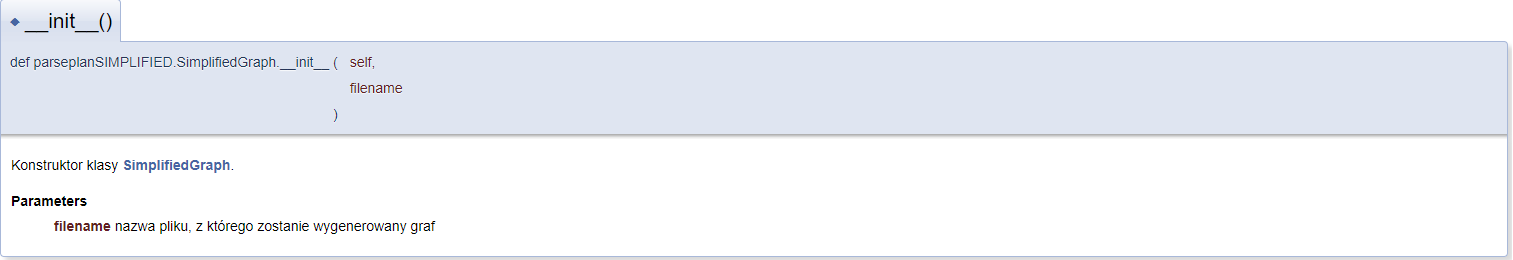
\includegraphics[scale=0.4]{OpisFunkcji}
        \centering
        \caption{Przykład opisu zaimplementowanej funkcji}
    \end{figure}

	\cleardoublepage

	\chapter{Testy}
\thispagestyle{chapterBeginStyle}

\section{15}
    \subsection{Wprowadzenie}
        Piętnastka (fr. taquin), znana również w Polsce o nazwie \textit{przesuwanka}, w zapisie często podawana przy pomocy liczbowego
        odpowiednika (15) jest grą w formie specyficznej
        układanki, której powstanie datuje się na koniec XIX wieku. Składa się ona z 
        15 klocków oraz ramki, pierwotnie drewnianej. Ramka zaprojektowana została specjalnie z myślą
        o pozostawieniu jednego wolnego miejsca, aby móc w łatwy sposób przesuwać klocki sąsiadujące z miejscem 
        pustym. Celem gry jest ułożenie klocków w określony sposób, najcześciej w porządku rosnącym czytając 
        od lewej do prawej rzędami, z określonego stanu początkowego. Częstym zabiegiem stosowanym przez 
        twórców ów układanki jest konwersja liczb na części obrazka, aby zachęcić do gry młodszych odbiorców.

        \begin{figure}[H]
            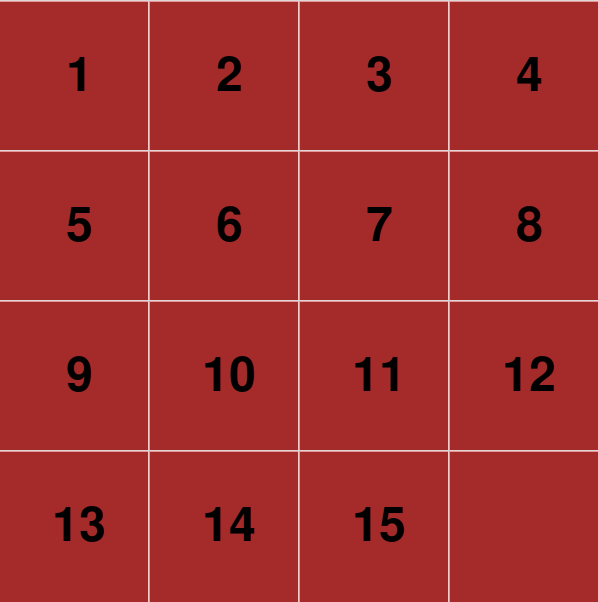
\includegraphics[scale=0.5]{15_ułożona}
            \centering
            \caption{Wygląd układanki piętnastki wygenerowany przy pomocy zaimplementowanej w ramach pracy warstwy graficznej}
        \end{figure}

        \begin{figure}[H]
            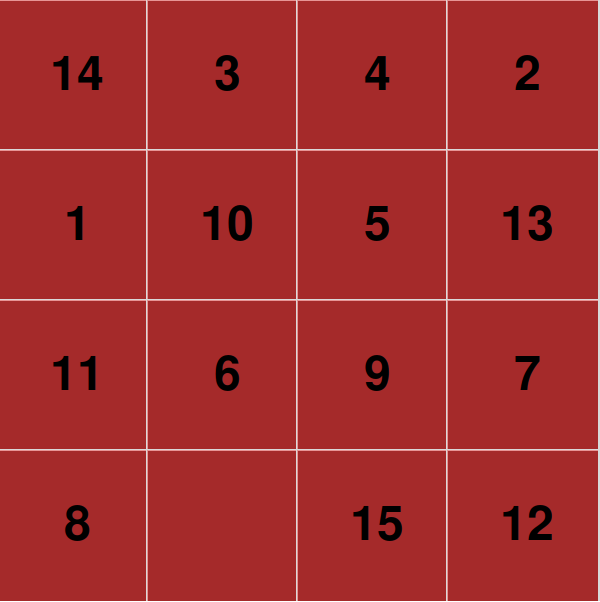
\includegraphics[scale=0.5]{15_losowe}
            \centering
            \caption{Losowa rozwiązywalna permutacja układanki}
        \end{figure}

        \begin{figure}[H]
            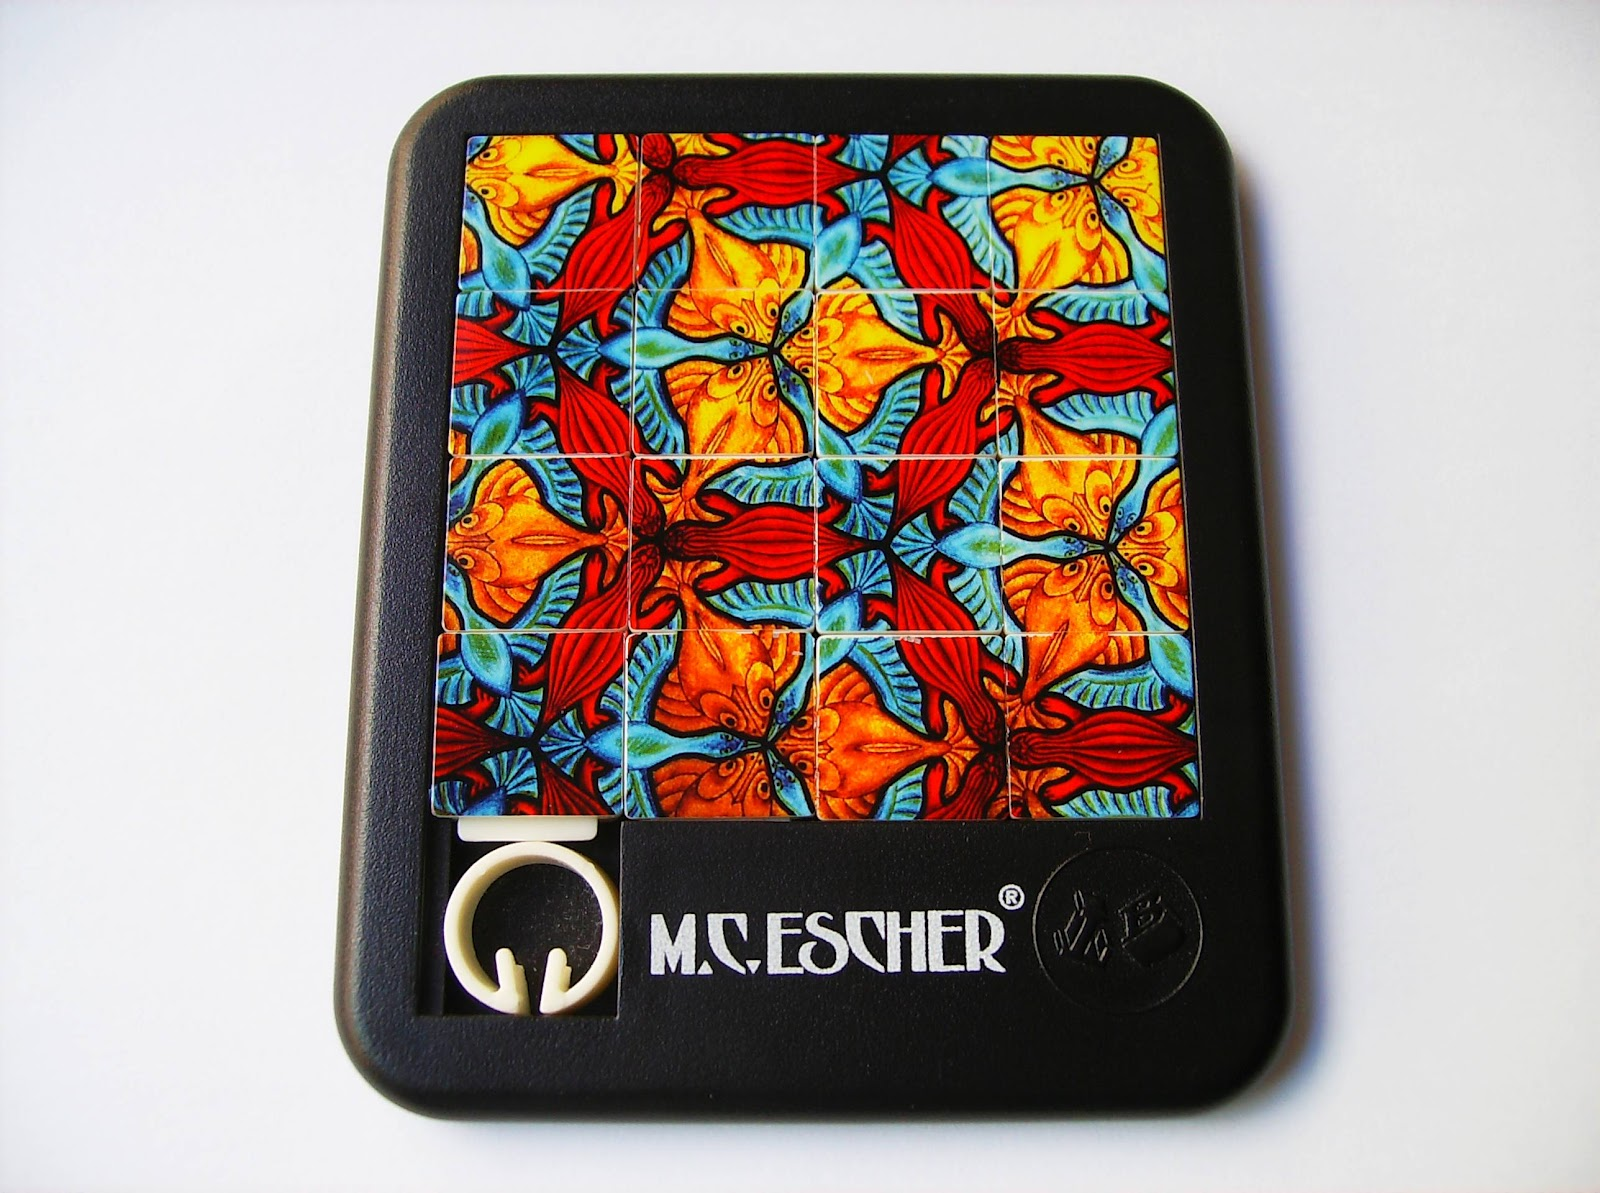
\includegraphics[scale=0.15]{15_obrazkowa}
            \centering
            \caption{Piętnastka w formie obrazkowej. Źródło: \url{http://mypuzzlecollection.blogspot.com/2012/08/mc-escher-birds-fish-and-turtles.html}}
        \end{figure}

    \subsection{Teoria}
        W 1878 roku amerykański wynalazca gier i zagadek (między innymi zagadek szachowych) \textbf{Samuel Loyd} ze względu na swój fach 
        nie przeszedł obojętnie koło piętnastki proponując ułożenie układu rosnącego z pozycji, która 
        od początkowej różniła się pozycjami jedynie dwóch klocków numerowanych odpowiednio 14 i 15 \cite{FifteenLoydProblem}.
        Problem ów stał się na tyle popularny, iż została wyznaczona nagroda 1000 dolarów dla osoby, której udałoby się 
        znaleźć prawidłowe rozwiązanie przygotowanego przez Pana Samuela problemu.

        Niemożliwość ułożenia problemu przez bardzo długi czas doprowadziła do pierwszych poważniejszych rozważań 
        nad z pozoru trywialną łamigówką. Efektem prac matematyków było parę zaskakujących wniosków, które ostatecznie doprowadziły 
        do udowodnienia, iż wyżej przedstawiona łamigłówka jest nierozwiązywalna.
        \begin{lemma}
            Nie wszystkie ustawienia początkowe piętnastki są możliwe do rozwiązania.\cite{Fifteen}
        \end{lemma}
        Wynika to z faktu, iż rozwiązywalne są jedynie rozwiązanie oo parzystej liczbie inwersji. Zagadka Pana Lyod'a jest 
        ustawieniem nieparzystym jeśli chodzi o inwersje. Prowadzi to do następującego wniosku:
        \begin{corollary}
            Istnieje $\frac{16!}{2}=10 461 394 944 000$ rozwiązywalnych ustawień. 
        \end{corollary}
        Dodatkową ciekawostką istotną z perspektywy wykonywanych testów jest minimalna liczba posunięć, którą należy wykonać, 
        aby z rozwiązywalnego stanu osiągnąć wcześniej wyznaczony cel. Mianem \textbf{boskiej liczby} w odniesieniu do przesuwanki
        określą się największą liczbę posunięć, którą trzeba osiągnąć, aby rozwiązać najtrudniejsze ułożeniem początkowe. Przy pomocy matematyki 
        naukowcy odnaleźli najtrudniejsze ustawienia oraz obliczyli ów liczbę, co zaprezentowano w następującym lemacie:
        \begin{lemma}
            \textbf{Boska liczba} dla 15-elementowej przesuwanki wynosi \textbf{80}. \cite{80Moves}
        \end{lemma}
        Oznacza to, iż maksymalna liczba kroków algorytmu w żadnym wypadku nie powinna przekroczyć liczby 80.

        W trakcie poniżej opisanego testu sprawdzono plany przesuwania odpowiednich klocków, aby w jak najmniejszej możliwej liczbie ruchów
        otrzymać odpowiedni stan końcowy, przy okazji sprawdzono osiągnięcia czasowe jak i porównano otrzymane wyniki z popularnymi herustykiami 
        spersonalizowanymi pod rozwiązywanie ów układanki.

    \subsection{Przykład}
        Na podstawie następującego przykładu zostanie przedstawiony schemat rozwiązywania układanki przez algorytm:
        \begin{figure}[H]
            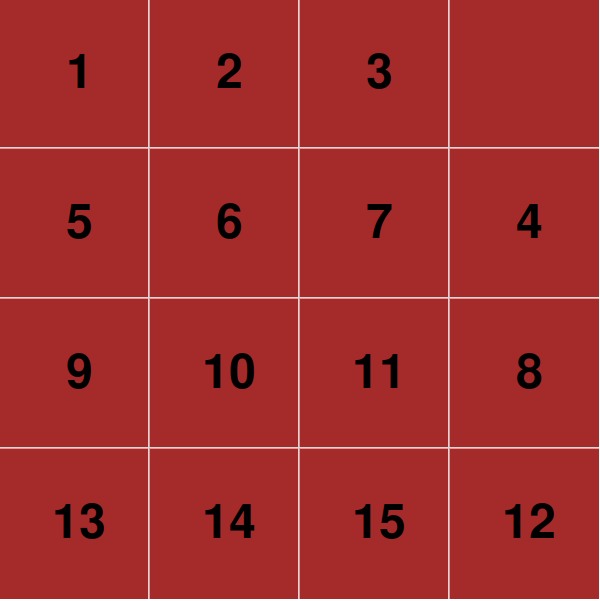
\includegraphics[scale=0.5]{15_przyklad}
            \centering
            \caption{Przykładowe startowe ułożenie przesuwanki}
        \end{figure}
        Algorytm buduje graf na podstawie jedynej zdefiniowanej w problemie akcji: przesuwania klocka. Robi to aż do momentu, gdy kafelki nie 
        będą ułożone w wczesniej zdefiniowanej kolejności. Dla zdefiniowanego powyżej przykładu w pierwszym kroku algorytm ma jedynie dwie możliwości 
        akcji aktywnych: zamiana klocka pustego z klockiem o numerze 3 lub klockiem o numerze 4. Na tej podstawie generuje kolejny poziom stanów. 
        Dla załączonego przykładu optymalnym rozwiązaniem jest odpowiednio zamiana pustego kafelka z kafelkami: 4,8,12, co zostało poprawnie 
        wyznaczone przez GRAPHPLAN. Poniżej przedstawiono zbiory akcji przeanalizowane przez algorytm w danym kroku jak i uproszczony graf planujący.

        \begin{figure}[H]
            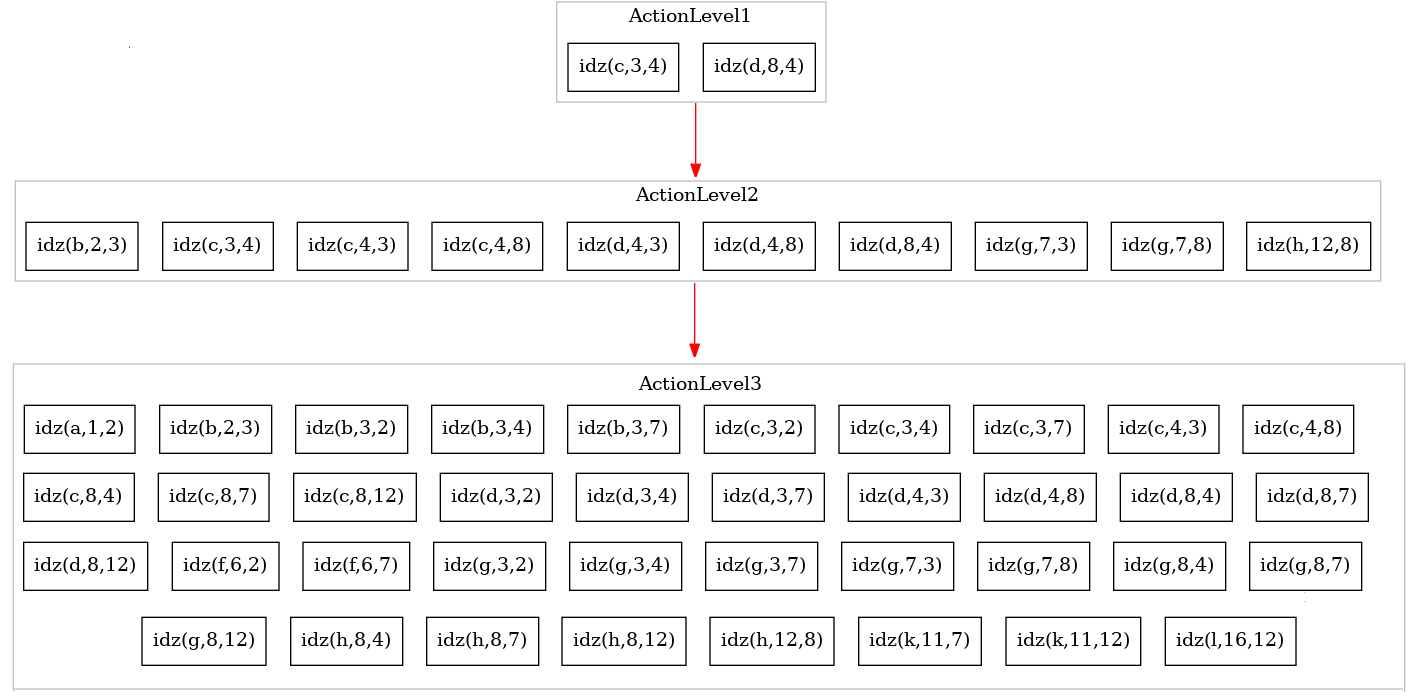
\includegraphics[scale=0.4]{15_zbiory_akcji}
            \centering
            \caption{Akcje rozpatrywane przez algorytm w danym kroku}
        \end{figure}

        \begin{figure}[H]
            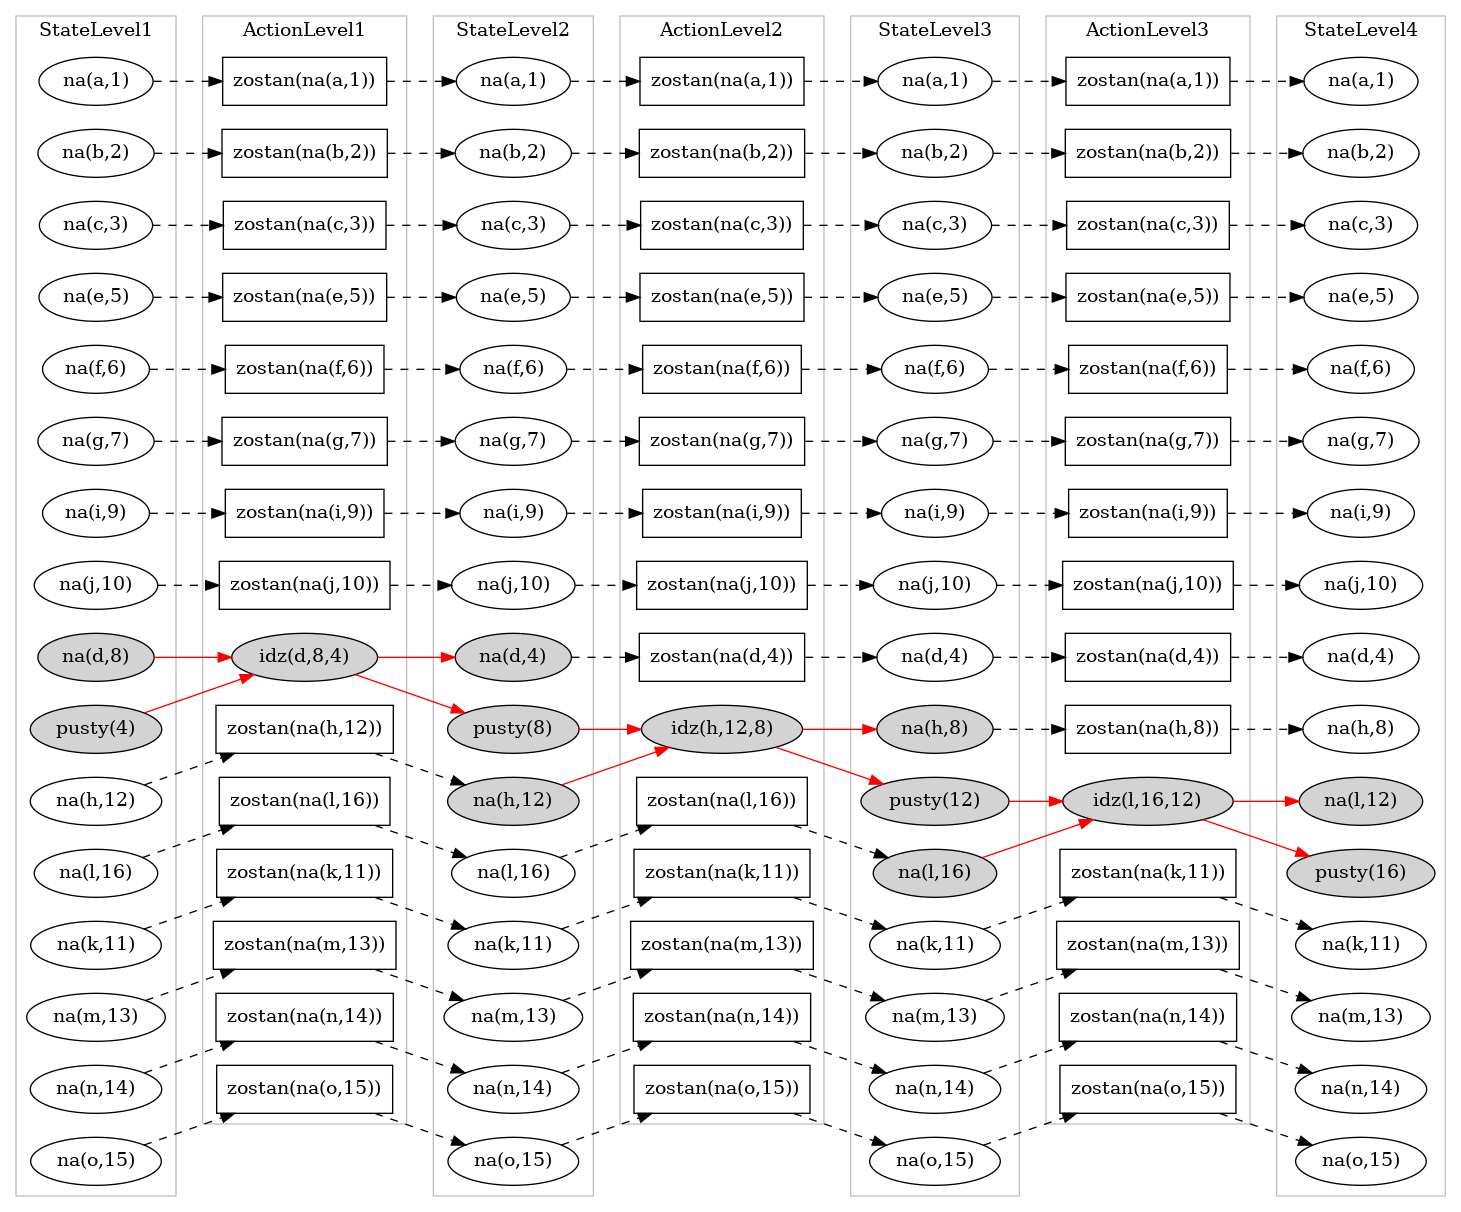
\includegraphics[scale=0.25]{15_graphplan}
            \centering
            \caption{Uproszczony graf planujący wygenerowany przez algorytm GRAPHPLAN przedstawiający stan każdego kafelka w danej warstwie. Węzły wypełnione 
            kolorem szarym obrazują stany, które są warunkami zajścia jak i efektami wykonywanej w danej warstwie akcji}
        \end{figure}

        \begin{figure}[H]
            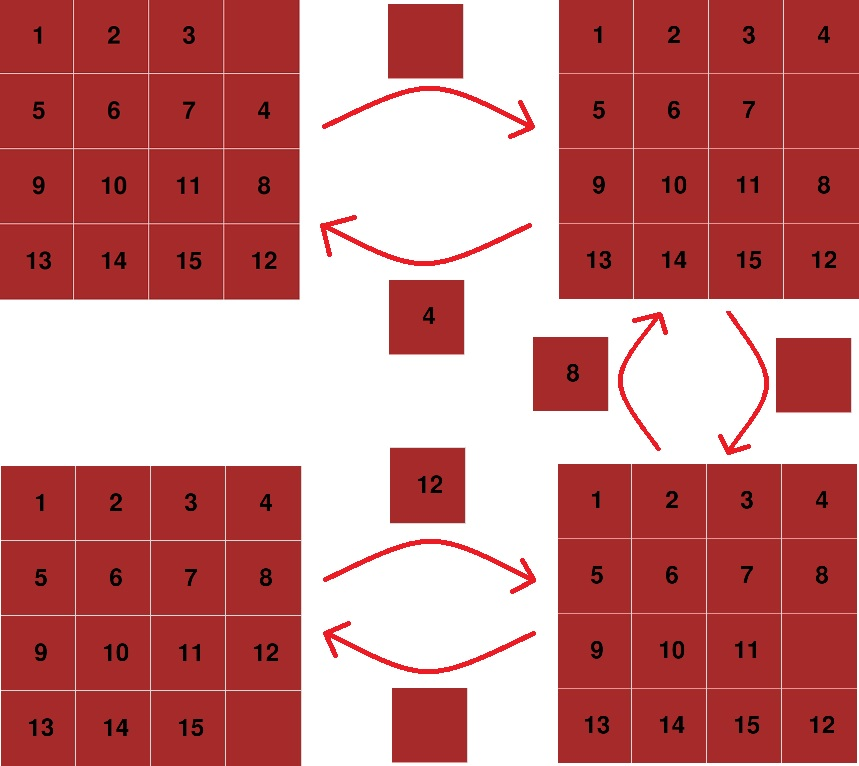
\includegraphics[scale=0.5]{15_zamiany}
            \centering
            \caption{Obrazowe rozwiązanie na podstawie wygenerowanego grafu}
        \end{figure}





    \subsection{Szczegóły implementacyjne}
    Ważnym jest, aby przedstawić omawiany świat zgodnie z wytycznymi ustalonymi przez język \textbf{STRIPS}. Z tego powodu należy dokładnie okreslić 
    każdą z istniejących w świecie relacji oraz poprawnie określić cel, jak i warunki początkowe.

    \subsection{Wyniki}

    \textbf{UWAGA:} Testy czasowe zaprezentowane w poniższych tabelach tyczą się osiągów samego algorytmu. Oznacza to, iż na czas wykonywania prób
    wyłączone zostały wszystkie poboczne funkcjonalności takie jak generowanie grafu, czy prezentowanie rozwiązania w formie graficznej. 
    Wykonanie poniższych badań w aplikacji może skutkować innymi wynikami, zwykle dłuższymi. Należy mieć to na uwadze przy potencjalnej 
    próbie odtwarzania badań.

    



    \subsection{Młodsza siostra- ósemka}

    \subsection{Wyniki dla 8}
    \subsection{Wnioski}
\section{CargoBot}
    \subsection{Wprowadzenie}
    \subsection{Przykład}
    \subsection{Szczegóły implementacyjne}
    \subsection{Wyniki}
    \subsection{Wnioski}
\section{Przemieszczanie w przestrzeni}
    \subsection{Wprowadzenie}
    \subsection{Przykład}
    \subsection{Szczegóły implementacyjne}
    \subsection{Wyniki}
    \subsection{Wnioski}
\section{Wieża Hanoi}
    \subsection{Wprowadzenie}
    \subsection{Przykład}
    \subsection{Szczegóły implementacyjne}
    \subsection{Wyniki}
    \subsection{Wnioski}
\section{Osiem Hetmanów}
    \subsection{Wprowadzenie}
    \subsection{Przykład}
    \subsection{Szczegóły implementacyjne}
    \subsection{Wyniki}
    \subsection{Wnioski}
	\cleardoublepage

	\chapter*{Podsumowanie}
\addcontentsline{toc}{chapter}{Podsumowanie}
\thispagestyle{chapterBeginStyle}

    Główny cel pracy, którym była implementacja algorytmu GRAPHPLAN wraz z programowaniem ograniczeń, został osiagnięty. Przy pomocy 
    nowego podejścia do programowania udało się ułatwić proces implementacji jak \\
    i przyśpieszyć czas tworzenia planu przez algorytm. Użytkownik 
    może skorzystać z wbudowanych światów w ramach interfejsu graficznego, bądź uruchomić program z poziomu linii komend przy okazji 
    definiując własne środowisko pracy. Na żądanie użytkownika generowane są odpowiednie grafy reprezentujące plan, jak i schemat 
    transformacji świata z wyszczególnieniem sytuacji, w jakiej znajduje się każdy stan początkowy na dowolnym etapie realizacji planu.
    W ramach sprawdzenia funkcjonalności wykonano testy na prostych, lecz obrazowych przykładach. Na ich podstawie można wywnioskować, iż GRAPHPLAN,
    zgodnie ze swoim założeniem generuje plany, które są optymalne, czyli składają się jak najmniejszej liczby kroków. Wykonując testy na 
    popularnej \textit{przesuwance} można było zauważyć, iż rozszerzanie grafu o nowe obiekty świata znacznie wpływa na długość wykonywania algorytmu. 
    Z tego powodu dokonano dodatkowych testów na zmniejszonej układance, z którą algorytm poradził sobie zdecydowanie lepiej. 

    Algorytm posiada szereg możliwości pozwalających na rozszerzenie jego funkcjonalności oraz zwiększenie efektywności generowania planów. W trakcie 
    implementacji można zastosować mechanizm \textit{podwójnego szukania}, który miałby za zadanie układać plan symultanicznie korzystająć z mechanizmu 
    cofania oraz, na wzór ludzki, wyszukując rozwiązania do przodu, dynamicznie zmieniając świat próbując w ten sposób uzyskać wyznaczony cel. \\
    Dodatkowo wartym uwagi jest fakt, iż
    w niektórych sytuacjach można zrezygnować z gwarancji najkrótszego możliwego rozwiązania na rzecz szybszego generowania planu. Ponadto 
    algorytm w swojej istocie bazuje głównie na relacji wzajemnego wykluczania. Istnieje możliwość, iż w zdefiniowanych światach istnieją inne informacje,
    które prowadziłyby do szybszego wyszukiwania odpowiedniego planu.

    Dalsze możliwe kierunki rozwoju oprogramowania to między innymi generowanie większej liczby grafów o różnych własnościach, które
    w dokładniejszy sposób prezentowałyby użytkownikowi esencję algorytmu, rozbudowa warstwy graficznej algorytmu pod kątem estetycznym jak i 
    pod kątem liczby światów w jakich użytkownik może generować plany.


	\cleardoublepage

	
	
	%%%%%%%%%%%%%%%%%%%%%%%%%%%%%%%%%%%%%%%%%%%%%%%%%%%%%%%%%%%%%%%%%%%%%%%%%%%%%%
	%%%%%%%%%%%%%%%%%%%%%%%%%%%%%%% BIBLIOGRAFIA %%%%%%%%%%%%%%%%%%%%%%%%%%%%%%%%%
	%%%%%%%%%%%%%%%%%%%%%%%%%%%%%%%%%%%%%%%%%%%%%%%%%%%%%%%%%%%%%%%%%%%%%%%%%%%%%%

	\pagestyle{bibliographyStyle}
	\bibliographystyle{plabbrv}
	\bibliography{literatura}
	\thispagestyle{chapterBeginStyle}
        \addcontentsline{toc}{chapter}{Bibliografia}
	\cleardoublepage
	
	%%%%%%%%%%%%%%%%%%%%%%%%%%%%%%%%%%%%%%%%%%%%%%%%%%%%%%%%%%%%%%%%%%%%%%%%%%%%%%
	%%%%%%%%%%%%%%%%%%%%%%%%%%%%%%%%% DODATKI %%%%%%%%%%%%%%%%%%%%%%%%%%%%%%%%%%%%
	%%%%%%%%%%%%%%%%%%%%%%%%%%%%%%%%%%%%%%%%%%%%%%%%%%%%%%%%%%%%%%%%%%%%%%%%%%%%%%
	
	\appendix
	\pagestyle{appendixStyle}
       \renewcommand{\appendixname}{Załącznik}
	
	\chapter{Zawartość płyty CD}
\thispagestyle{chapterBeginStyle}
\label{plytaCD}

W tym rozdziale należy krótko omówić zawartość dołączonej płyty CD.


	
	\cleardoublepage

\end{document}

